\section{Evaluation der Integrations- und Bereitstellungs-Tools unter Anwendung des Analytischen Hierarchieprozesses}
\label{sec:AHP}
\subsection{Definition der Entscheidungskriterien}
 Die zur Durchführung des AHP-Verfahrens benötigten Daten werden neben einer Literaturrecherche ebenfalls mittels Experteninterviews erhoben. Für die Experteninterviews wird ein Gremium aus acht Mitarbeitenden der SAP zusammengestellt (s. Anhang \ref{sec:Expertenmaterialien}). Diese sind jeweils in verschiedenen Bereichen der Cloud-Fullstack-Entwicklung, Test-Management, Product Management sowie in der Softwarearchitektur spezialisiert. Somit kann Expertise von Spezialisten verschiedener Fachbereiche konsolidiert und Anforderungen aller an der Entwicklung, Bereitstellung sowie an dem Betrieb von Software beteiligten Stakeholdern erfasst werden. Zur Festlegung der Entscheidungskriterien wird eine induktive Kodierung der Expertengespräche durchgeführt (s. Anhang \ref{sec:kodierung}). Dabei werden aus besonders häufig von Experten genannten Aspekten systematisch Kategorien abgeleitet. Diese umfassen insbesondere Elemente, welche die in vergangenen Kundenprojekten hervorgegangenen Anforderungen an eine CI/CD-Pipeline widerspiegeln. Neben den in externen Projekten anfallenden Anforderungen werden bei der Kriterienbildung ebenfalls interne, von der SAP zur Bereitstellung von Standardsoftware festgelegte Bestimmungen berücksichtigt. Obwohl Kunden bei der Entwicklung eigener Services nicht zur Einhaltung dieser Richtlinien verpflichtet sind, erlaubt eine Berücksichtigung dieser Aspekte die Festlegung eines Optimalzustands. Die bei der induktiven Kodierung erhobenen Kategorien werden anschließend ebenfalls als Entscheidungskriterien im AHP-Verfahren wiederverwendet.\\ Die mit dieser Vorgehensweise erhobenen Entscheidungsalternativen sind der Tabelle \ref{fig:AHP_E} zu entnehmen. 
 Auf der obersten Ebene des AHP-Entscheidungsbaums werden neun Kategorien definiert. Das erste Kriterium ist \textbf{Funktionalität} (K1). Diese Kategorie umfasst verschiedene innerhalb des CI/CD-Workflows benötigte funktionale Spezifikationen. So sollte eine Pipeline laut Experte 1 etwa dazu in der Lage sein, Anwendungen zu testen, Code-Analysen durchzuführen und IT-Services auf der Cloud-Plattform bereitzustellen \cite[Z. 72 ff.]{ProductOwnerSAPBTPProd&Infra.}. Angesichts der Vielfältigkeit des Entscheidungskriteriums Funktionalität wird eine Untergliederung in verschiedene Subkriterien vorgenommen. 
 \begin{center}
	\begin{table}[H]
		\centering
		\scalebox{0.5}{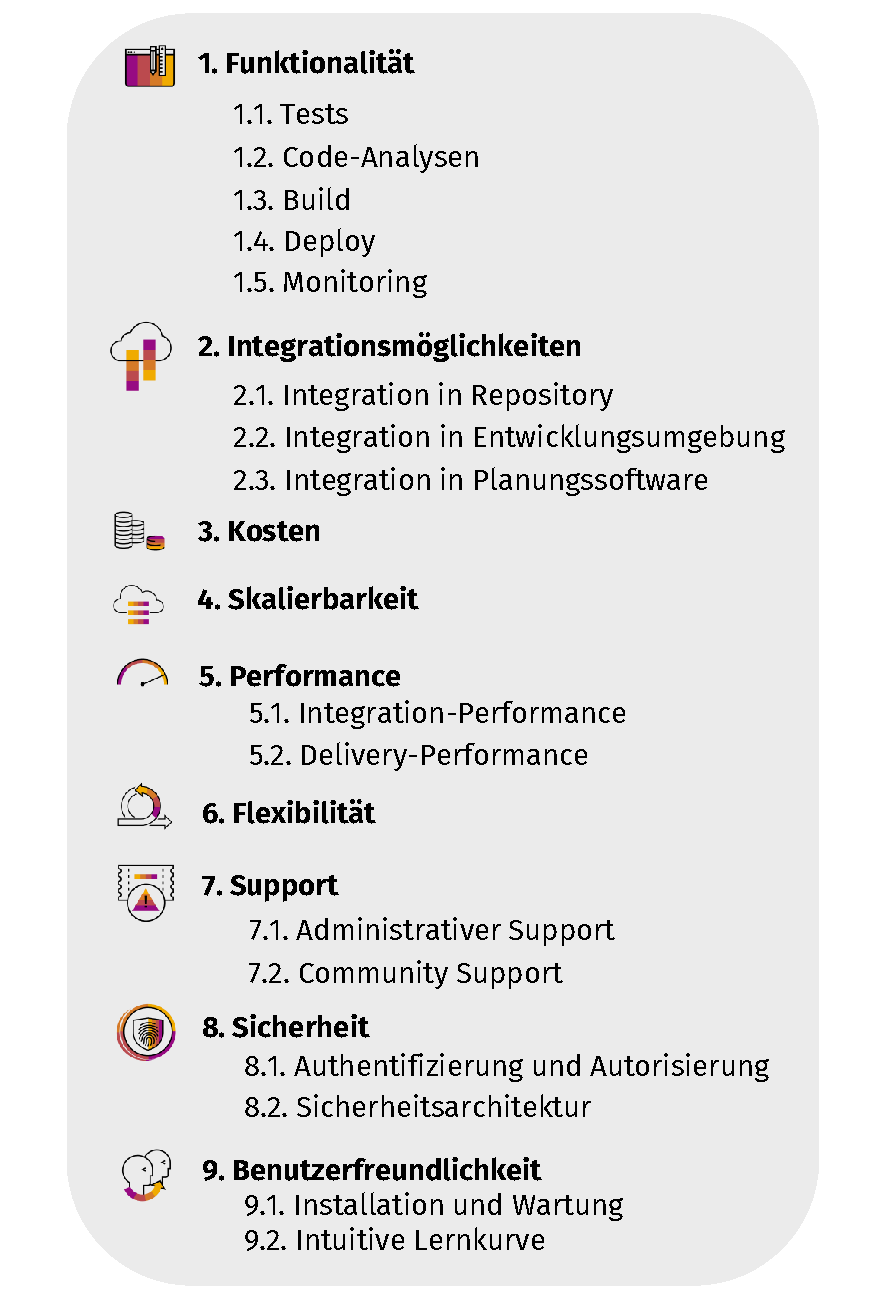
\includegraphics{AHP_E}}
		\caption[AHP-Entscheidungsstruktur zur Bewertung von CI/CD-Pipelines]{AHP-Entscheidungsstruktur zur Bewertung von CI/CD-Pipelines. Eigene Darstellung.}
		\label{fig:AHP_E}
	\end{table}
\end{center}
\vspace*{-15mm}
In Kriterium K1.1 wird dabei die Unterstützung automatisierter Unit-Tests evaluiert \cite[Z. 72 ff.]{ProductOwnerSAPBTPProd&Infra.}. Von der SAP werden diesbezüglich Produktstandards vorgegeben. Diese stützen sich auf \textit{ISO 9001}, eine internationale Norm für Qualitätsstandards. Im Kontext der Softwareentwicklung verlangt diese, eine für neue Funktionalitäten kontinuierlich und automatisiert durchgeführte Prüfung \cite[Z. 65 ff.]{TestDeveloperSAPHyperspaceAdoption&Onboarding.b}. Dies umfasst eine Abwicklung von Unit-, Integration-, E2E-Test sowie Regression-Tests für Backend sowie Frontend. Im Rahmen der SAP-Produktstandards werden dabei verschiedene Test-Tools empfohlen. Hinsichtlich der Entwicklung von SAP-CAP-Node-Anwendungen wird die Durchführung von Unit-Tests mittels Jest bzw. Mocha und Integration-Tests mittels Newmann vorgeschlagen. Für die Programmierung mit SAP UI5 sind hingegen Unit-Tests mittels Q-Unit, Integration-Tests mittels OPA5 und E2E-Tests mittels WDI5 vorgesehen \cite[Z. 66 ff.]{TestDeveloperSAPHyperspaceAdoption&Onboarding.b}. Für Regression-Tests wird hingegen kein spezifisches Test-Framework verwendet. In diesem Zusammenhang wird lediglich überprüft, ob eine erneute Validierung bereits bestehender Softwarekomponenten durchführbar ist. In Kriterium K1.2 wird die Kompatibilität verschiedener \textit{Code-Analyse-Tools} untersucht \cite[Z. 72 ff.]{ProductOwnerSAPBTPProd&Infra.}. Es wurde gezielt eine Trennung dieser Kategorie mit dem Kriterium K1.2 (Tests) vorgenommen. Während Tests eine funktionale Erfüllung der Anforderung evaluieren, werden  mit den Analysen Code-Qualitätsstandards der entwickelten Funktionalitäten untersucht. Dabei wird evaluiert, ob statische Code-Analysen, Security- sowie Performance-Überprüfungen von den CI/CD-Pipelines unterstützt werden. Laut Experte 3 werden für statische Code-Analysen gemäß Produktstandards der SAP Lint sowie SonarQube verwendet \cite[Z. 44 ff.]{ProductManagerSAPHyperspaceSecurityTools.}. Zur Durchführung von Sicherheitsüberprüfungen wird für SAP-CAP-Node-Anwendungen Checkmarx verwendet, während für SAP UI5 DASTER zum Einsatz kommt. Für Performance-Tests wird das Tool JMeter verwendet. In der Kategorie K1.3 werden die \textit{Build-Funktionalitäten} der CI/CD-Pipeline-Tools evaluiert \cite[Z. 71 ff.]{ProductOwnerSAPBTPProd&Infra.}. Sowohl für SAP-UI5- als auch SAP-CAP-Node-Anwendungen wird bei der Kompilierung das \textit{Multi-Target-Application-Konzept (\acs{MTA}-Konzept)} verwendet. Die MTA ist eine Applikation, z.B. ein Microservice eines CEs, welche aus verschiedenen Modulen besteht. Diese Module umfassen typischerweise die durch einen Microservice bereitgestellte API oder eine von der Applikation verwendete Datenbank. Eine MTA besitzt dabei einen sog. \textit{MTA-Deskriptor}, welcher die zur Kompilierung benötigten Konfigurationen enthält. Diese mit dem MTA-Konzept vorgesehene Modul-Bündelung ermöglicht somit, dass komplexe aus verschiedenen Komponenten bestehende Microservices in einer einzigen Datei beschrieben werden können \cite{.20230405b}. Da für das Kompilieren von MTAs das Build-Tool Make benötigt wird, wird evaluiert, ob dieses durch die Pipeline-Tools unterstützt wird. Laut Experte 1 ist weiterhin essenziell, dass Artefakt-Repositories durch die Pipeline-Tools unterstützt werden \cite[Z. 15 ff.]{ProductOwnerSAPBTPProd&Infra.}. Eine MTA kann von verschiedenen externen Ressourcen abhängig sein. Diese sind in einem Artefakt-Repository verwaltete Komponenten, welche bei der Entwicklung neuer Microservices wiederverwendet werden können \cite[Z. 40 ff.]{ProductOwnerSAPBTPProd&Infra.}. Diese Komponenten werden während des Build-Prozesses von der CI/CD-Pipeline aus den Artefakt-Repositories geladen und kompiliert. Aus diesem Grund ist es von bedeutendem Mehrwert, wenn CI/CD-Tools entweder über ein integriertes Artefakt-Repository verfügen oder die Möglichkeit der Einbindung externer Versionsverwaltungssysteme besteht. Ein weiterer für CEs essenzieller Build-Aspekt ist die Unterstützung von Kompilierungs-Tools für Docker-Container. Docker-Container sind portable und isolierte Laufzeitumgebungen, welche alle notwendigen Abhängigkeiten und Ressourcen einer Anwendung beinhalten. Somit können virtualisierte Umgebungen mit benötigten Frameworks und Tools bereitgestellt werden, ohne dabei eine gesamte Infrastruktur manuell konfigurieren zu müssen. \cite{Arora.20200504}. In Kriterium K1.4 werden die \textit{Deploy- und Release-Funktionalitäten} der CI/CD-Tools untersucht \cite[Z. 73 ff.]{ProductOwnerSAPBTPProd&Infra.}. Dabei wird evaluiert, ob die Pipelines neben dem Ausrollen von Software auf die Cloud-Foundry-Laufzeitumgebung ebenfalls verschiedene Bereitstellungsstrategien unterstützen (z.B. Blue/Green-Deployment s. Kap. \ref{sec:Bereitstellungs_Strategien}). Des Weiteren wird erörtert, ob mit den CI/CD-Pipelines eine Bereitstellung in das \ac{SAP CTM} möglich ist.
Das SAP CTM kann als zusätzliche Schicht im CI/CD-Prozess verbaut werden (s. Abb. \ref{fig:CTM}). Experte 2 merkt an, dass dieses System dabei insbesondere innerhalb komplexer ERP-Landschaften zur Optimierung der Bereitstellungsprozesse führen kann (weitere Details in Kap. \ref{sec:Bewertung})\cite[Z. 65 ff.]{ProductManagerSAPHyperspaceCICD.}. In Kategorie K1.5 wird die \textit{Monitoring-Funktionalität} der verschiedenen CI/CD-Pipelines untersucht \cite[Z. 37 ff.]{ProductManagerSAPHyperspaceCICD.}. In diesem Zusammenhang erfolgt eine Bewertung der Überwachbarkeit der CI/CD-Tools. Für interne Projekte wird dabei i.d.R. das SAP-Partner-Tool Splunk verwendet \cite[Z. 74 ff.]{ProductManagerSAPHyperspaceCICD.}. Damit lassen sich verschiedene Metriken, wie Build-Zeiten, Performance-Checks oder Fehlerquoten verschiedener Pipelines in einem zentralisierten Dashboard visualisieren. Da CI/CD-Pipelines im Rahmen dieser Arbeit insbesondere für externe Kundenprojekte evaluiert werden, ist innerhalb dieses Kriteriums ebenfalls eine Betrachtung von externen Open-Source-Tools vorgesehen. Zur Eingrenzung des Bewertungsumfangs, fokussiert sich die Open-Soruce-Untersuchung ausschließlich auf das Kibana-Dashboard, welches aufgrund seiner weiten Verbreitung bei Kunden von besonderer Relevanz ist \cite[Z. 74 ff.]{ProductManagerSAPHyperspaceCICD.}.\\In Kategorie K2 werden die \textbf{Integrationsmöglichkeiten} der Pipelines untersucht. In dem Subkriterium \textit{Integrationsmöglichkeiten von Repositories (Kategorie K2.1)} wird evaluiert, ob sich das Repository in die Pipeline integrieren lässt \cite[Z. 89 ff.]{ProductOwnerSAPBTPProd&Infra.}. Damit können bestimmte Ereignisse, wie Push-Mitteilungen bei Code-Änderungen automatisiert an die CI/CD-Pipeline übermittelt werden, was in einer unmittelbarer Auslösung des Integrations- bzw. Bereitstellungs-Workflows der CI/CD-Pipeline resultiert. Bei der Bewertung wird ein besonderes Augenmerk darauf gelegt, dass häufig verwendete Repositories problemlos in die Pipeline integrierbar sind. Da in der Literatur diesbezüglich keine öffentlichen Statistiken zugänglich sind, wird auf empirische Einschätzungen der Experten zurückgegriffen. So wurden nach Beurteilung des Experten 3 innerhalb interner und externer Projekte am häufigsten GitHub, GitLab und BitBucket verwendet \cite[Z. 95 ff.]{TestDeveloperSAPHyperspaceAdoption&Onboarding.}. In Kriterium K2.2 werden die \textit{Integrationsmöglichkeiten von Entwicklungsumgebungen} untersucht \cite[Z. 93 ff.]{ProductOwnerSAPBTPProd&Infra.}. Die Integration-Pipeline kann unmittelbar während des Entwicklungsprozesses aus der Entwicklungsumgebung gestartet werden. Auf diese Weise wird sichergestellt, dass Entwickler Feedback in noch kürzeren Zeitabständen erhalten als bei einer ausschließlichen Integration der Pipeline in das Repository. Die Bewertung bezieht sich dabei ausschließlich auf SAP-UI5- sowie SAP-CAP-Node-Entwicklungsumgebungen. Dazu gehören Microsoft Visual Studio Code, \ac{SAP BAS} sowie Eclipse. In Kriterium K2.3 wird die \textit{Integrationsmöglichkeit von Planungssoftware} untersucht \cite[Z. 96 ff.]{TestDeveloperSAPHyperspaceAdoption&Onboarding.}. Dazu gehören Projektmanagement-Tools wie Jira. Laut Experte 4 ermöglicht die Integration einer solchen Planungssoftware, Projektmanager eine erhöhte Transparenz über den Bereitstellungs-Workflow aller zu implementierender Arbeitselemente zu erhalten \cite[Z. 96 ff.]{TestDeveloperSAPHyperspaceAdoption&Onboarding.}. Auf diese Weise kann der CI/CD-Status eines Backlog-Items unmittelbar über die Planungssoftware eingesehen werden. Da die Wahl eines Pipeline-Tools i.d.R. nicht von der Unterstützung eines bestimmten Projektmanagement-Tools abhängig gemacht wird, erfolgt lediglich eine Untersuchung der generellen Integrationsfähigkeit von Planungssoftware \cite[Z. 96 ff.]{TestDeveloperSAPHyperspaceAdoption&Onboarding.}.\\In Kriterium K3 erfolgt die Evaluation der \textbf{Kosten} \cite[Z. 42 ff.]{ProductManagerSAPHyperspaceCICD.}. Mit diesem Entscheidungskriterium werden die durch die CI/CD-Pipelines verursachten \textit{\ac{TCO}} evaluiert. TCO beschreiben den Geldbetrag, welchen ein Unternehmen während des gesamten Lebenszykluses einer Investition, also von Beschaffung bis zur vollständigen Entsorgung, aufbringen muss \cite[4]{Ellram.1993}. Da für die zu untersuchenden Pipeline-Tools keine vergleichbaren Kostenmodelle verfügbar sind, werden die Kosten ausschließlich qualitativ beurteilt. Somit werden Aspekte wie Einrichtungs-, Betriebs- sowie Wartungsaufwendungen evaluiert. \\In Kriterium K4 wird die \textbf{Skalierbarkeit} der CI/CD-Pipelines analysiert \cite[Z. 69 ff.]{ProductOwnerSAPBTPProd&Infra.}. Hierbei werden die Pipelines auf horizontale sowie vertikale Skalierbarkeit untersucht. Die horizontale Skalierbarkeit ermöglicht eine parallele Durchführung mehrerer Builds. Gerade bei einer hohen Anzahl gleichzeitiger Hauptzweigintegrationen birgt dies einen bedeutenden Mehrwert. Die vertikale Skalierung bezieht sich auf die Erhöhung der Ressourcen einer einzigen Pipeline-Instanz. Laut Experte 1 kann die CI/CD-Pipeline so dynamisch an die sich ändernden Leistungsanforderungen angepasst werden \cite[Z. 74 ff.]{ProductOwnerSAPBTPProd&Infra.}. \\In Kriterium K5 wird die \textbf{Performance} der Pipelines verglichen \cite[Z. 35 ff.]{ProductManagerSAPHyperspaceCICD.}. Dabei wird die zur Prozessierung des CI/CD-Workflows benötigte Zeit der zu untersuchenden Tools anhand eines für die Arbeit implementierten CEA-Prototyps evaluiert (s. \ref{fig:Szenario}). Im Rahmen dieser Gegenüberstellung wird eine Unterscheidung zwischen der Integration- bzw. Delivery-Zeit realisiert. Die Integration-Zeit bezeichnet den Zeitraum, welcher von der Einführung eines Feature-Branches bis zur vollständigen Konsolidierung in den Hauptzweig benötigt wird. Dabei werden für die Microservices Validierungen, wie Unit- sowie Integration-Tests, welche für gewöhnlich in einem CI-Prozess abgewickelt werden, implementiert und in die Pipeline eingebunden. Die Delivery-Zeit beschreibt die Zeitspanne, welche von der Freigabe des Hauptzweigs bis zur Bereitstellung der Software auf die Cloud-Plattform benötigt wird. Dabei werden ebenfalls CD-typische Schritte, wie E2E-Tests und Code-Analysen implementiert und in die Pipelines integriert.\\ In Kriterium K6 wird die \textbf{Flexibilität} der verschiedenen Pipelines evaluiert \cite[Z. 70 ff.]{ProductOwnerSAPBTPProd&Infra.}. Eine bedeutende Dimension der Flexibilität ist die uneingeschränkte Konfigurierbarkeit der Pipelines. So sollte eine Pipeline laut Experte 1 etwa keinerlei Beschränkungen in Bezug auf Anzahl und Reihenfolge der im CI/CD-Workflow durchzuführenden Schritte besitzen \cite[Z. 70 ff.]{ProductOwnerSAPBTPProd&Infra.}. Weiterhin wird evaluiert, ob die Pipelines einen modularen Aufbau unterstützen. Um die aus einer Bereitstellungslandschaft mit einer Vielzahl an CI/CD-Pipelines resultierende Komplexität zu reduzieren, sollten Pipelines aus modularen wiederverwendbaren Komponenten zusammengesetzt werden können. Sofern eine neue Pipeline erforderlich ist, besteht die Möglichkeit, diese ohne hohen Implementierungsaufwand aus den wiederverwendbaren CI/CD-Komponenten zu konstruieren. Ein weiterer für die Flexibilität der Pipelines essenzieller Aspekt, ist die Unterstützung von Plug-ins. Da mit diesen ebenfalls nicht im Standard verfügbare Funktionalitäten in die Pipeline integriert werden können, besteht für Entwicklungsabteilungen die Möglichkeit flexibel auf Anforderungen aller Stakeholder zu reagieren.\\ In Kriterium K7 wird der für die CI/CD-Pipelines bereitgestellte \textbf{Support} evaluiert. Im Hinblick auf den \textit{Administrativen Support (K7.1)} wird geprüft, ob die Pipeline-Anbieter Unterstützung bei der Einrichtung, Konfiguration sowie Problembehebung der CI/CD-Tools bieten \cite[Z. 44 ff.]{ProductManagerSAPHyperspaceCICD.}. Dies ist insbesondere dann hilfreich, wenn der Umgang mit den Pipelines einen hohen Grad an Expertise erfordert. Des Weiteren wird evaluiert, ob Schulungen sowie Informationsmaterial verfügbar sind. Somit soll der Wissenstransfer und das Verständnis der involvierten Technologien und Prozesse innerhalb der Entwicklungsteams gefördert werden. Ein weiterer wesentlicher Aspekt ist die Verfügbarkeit von Updates. Durch kontinuierliche Updates kann sichergestellt werden, dass die Pipeline stets auf dem neuesten Stand der Technik ist. Im Kontext des \textit{Community-Supports (Kriterium K7.2)} wird geprüft, ob öffentliche Foren existieren, in welchen Anwender Fragen stellen und Probleme diskutieren können \cite[Z. 46 ff.]{ProductManagerSAPHyperspaceCICD.}. Die Qualität des Community-Supports hängt dabei i.d.R. von dem Kontributionsmaß der Pipeline-Tools innerhalb der Foren ab. Somit wird als Bewertungsgrundlage die Anzahl der zu einer CI/CD-Pipeline abgesetzten Posts verglichen. Als Referenzquelle dient hierbei das größte Entwicklerforum Stack Overflow \cite{StackOverflow.20230403}.\\ In dem Kriterium K8 wird die \textbf{Sicherheit} der CI/CD-Pipelines untersucht \cite[Z. 79 ff.]{ProductOwnerSAPBTPProd&Infra.}. Um unerwünschte Zugriffe zu vermeiden, sollte die CI/CD-Pipeline ein Authentifizierungs- und Autorisierungskonzept unterstützen. Besonders vorteilhaft ist dabei die Einbindung zentralisierter Drittanbieter, wie der SAP Identity Provider oder GitHub. Ein weiterer unter dem Kriterium der Sicherheit evaluierter Aspekt ist ebenfalls die Systemsicherheit. Dazu gehört neben dem Schutz der Systemintegrität ebenfalls die Ausfallsicherheit.\\ In Kriterium K9 wird die \textbf{Benutzerfreundlichkeit} der CI/CD-Pipelines untersucht. Hinsichtlich der \textit{Installation und Wartung (Kriterium K9.1)} ist es dabei besonders vorteilhaft, wenn das Aufsetzen und Einrichten des Pipeline-Systems nicht selbst übernommen werden muss, sondern unmittelbar als Service bereitgestellt wird \cite[Z. 67 ff.]{ProductOwnerSAPBTPProd&Infra.}. Auch der für die Implementierung und Konfiguration der Pipelines benötigte Aufwand sollte so gering wie möglich sein (\textit{intuitive Bedienbarkeit}) \cite[Z. 67 ff.]{ProductOwnerSAPBTPProd&Infra.}. Um die Abhängigkeit einer Abteilung von hochqualifizierten DevOps-Spezialisten zu verringern, kann es
einen Mehrwert darstellen, wenn Pipelines nicht mittels Programmiersprachen, sondern über intuitive Benutzeroberflächen konfigurierbar sind. 
\subsection{Festlegung der Bewertungsmetriken}
\label{sec:Metriken}
In diesem Abschnitt erfolgt die Festlegung der Bewertungsmetriken. Dabei ist eine Bewertung von null bis vier Punkte vorgesehen. Eine Bewertung mit vier Punkten wird vergeben, wenn eine CI/CD-Pipeline signifikant zur Zielerreichung eines Kriteriums beiträgt, während eine Bemessung von null Punkten eine unterdurchschnittliche Leistung impliziert. Die Vergabe von null Punkten stellt sicher, dass ein Kriterium, falls das zu bewertende Tool keinen Mehrwert birgt, nicht zur Erhöhung der Gesamtbewertung beiträgt. 
Für qualitative, in dem Entscheidungs-Framework zu betrachtende Kriterien wird eine gewichtende Bewertung vorgenommen:\\
\begin{tabular}{ l l }
	\textbf{\textbullet O Punkte:} & Ausschließlich Nachteile \\
	\textbf{\textbullet 1 Punkt:} & Nachteile überwiegen Vorteilen\\
	\textbf{\textbullet 2 Punkte:} & Vorteile und Nachteile gleichgewichtig\\
	\textbf{\textbullet 3 Punkte:} & Vorteile überwiegen Nachteilen\\
	\textbf{\textbullet 4 Punkte:} & Ausschließlich Vorteile\\
\end{tabular}\\\\
Dabei erfolgt eine Abwägung der Vor- und Nachteile, welche sich aus der Nutzung einer bestimmten Pipeline ergeben. Auf diese Weise kann bei der Bewertung ebenfalls argumentativ auf die in einer CEA vorliegenden Anforderungen eingegangen werden. Aufgrund des qualitativen Evaluationsdesigns wird diese Metrik für die Kriterien \textit{Funktionalität (K1)}, \textit{Integrationsmöglichkeiten (K2)}, \textit{Skalierbarkeit (K4)}, \textit{Flexibilität (K5)}, \textit{Administrativer Support (K7.1)}, \textit{Sicherheit (K8)} und \textit{Benutzerfreundlichkeit (K9)} angewendet. Da für die Pipelines unterschiedliche  Preismetriken festgelegt sind, kann das Kriterium \textit{Kosten (K3)} ebenfalls ausschließlich anhand der qualitativen Metrik bewertet werden. Für das quantitative Kriterium \textit{Performance (K5)} wird eine divergierende Metrik definiert:\vspace{2mm}\\
\begin{tabular}{ l l }
	\textbf{\textbullet O Punkte:} & 75 Prozent oder mehr über dem niedrigsten Wert \\
	\textbf{\textbullet 1 Punkt:} & 50 Prozent bis 75 Prozent über dem niedrigsten Wert\\
	\textbf{\textbullet 2 Punkte:} & 25 Prozent bis 50 Prozent über dem niedrigsten Wert\\
	\textbf{\textbullet 3 Punkte:} & 0 Prozent bis 25 Prozent über dem niedrigsten Wert\\
	\textbf{\textbullet 4 Punkte:} & Niedrigster Wert\\
\end{tabular}\\\\
Mithilfe dieser Metrik lassen sich die relativen Integration- bzw. Delivery-Zeiten der CI/CD-Pipelines vergleichend betrachten. Indem der höchste Wert als Bezugsgröße verwendet wird, ermöglicht sich ein Vergleich in Relation zur besten Entscheidungsalternative. Das vorliegende Evaluationsdesign erweist sich dabei als besonders vorteilhaft, da dieses eine Bewertung ermöglicht, ohne vorab spezifische Referenzwerte festzulegen. In Kriterium K7.2 (\textit{Community-Support}) ist ebenfalls eine quantitative Bewertung vorgesehen. Dabei wird die Anzahl der abgesetzten Blog-Posts zu einer CI/CD-Lösung evaluiert. Hierbei erfolgt eine inverse Bewertung nach der zuvor definierten qualitativen Metrik. So werden vier Punkte für die höchste Blog-Post-Anzahl vergeben. Für die restlichen Bewertungen wird invers nach den in der qualitativen Metrik definierten Abstufungen benotet. 

\subsection{Ermittlung der Gewichtungsfaktoren}
\label{sec:Gewichtung}
Zur Bestimmung einer optimalen, auf die Präferenzen der Entscheidungsträger ausgerichteten CI/CD-Pipeline wird eine Gewichtung der Bewertungskriterien vorgenommen. Die Gewichtung wird dabei von einem Expertengremium, bestehend aus fünf Mitarbeitenden der SAP, durchgeführt. Dieses umfasst einen Softwarearchitekten, einen Backend- sowie Frontend-Test-Entwickler, einen Fullstack-Entwickler und einen Product Manager (s. Anhang \ref{sec:Expertengewichtung}). Dabei wird die in Kapitel \ref{sec:meth_ahp} erläuterte Paarvergleichgewichtung von jedem Experten zunächst eigenständig durchgeführt. Im Anschluss erfolgt die Berechnung des Mittelwertes aller Einzelgewichtungen. Mit diesem Vorgehen wird gewährleistet, dass bei der Gewichtung divergierende Anforderungen und Bedürfnisse aller an dem Bereitstellungsprozess von Software beteiligten Stakeholder adäquat berücksichtigt werden.\\   
In Abb. \ref{fig:AHP_G} werden die lokalen und globalen Durchschnittsgewichtungen der AHP-Entscheidungskriterien dargestellt.
Die Experten legen dabei auf unterschiedliche Aspekte Wert. So ist für den Softwarearchitekten die von den Pipelines bereitgestellte Funktionalität von hoher Bedeutung. Innerhalb dieses Kriteriums besonders ausschlaggebend ist für diesen Experten dabei die Unterstützung verschiedener Test-Frameworks. Nach Auffassung des Architekten besteht zwar die Möglichkeit, Tests manuell und unabhängig von einer Pipeline auszuführen. Allerdings gestaltet sich dabei die Überwachung der Einhaltung dieser Testrichtlinien als sehr herausfordernd \cite[Z. 18 ff.]{SoftwareArchitektSAPDTSIntegration.}. Bei einer CEA ist es üblich, dass eine hohe Bandbreite verschiedener Programmier-Frameworks eingesetzt wird \cite[Z. 13 ff.]{SoftwareArchitektSAPDTSIntegration.}. Aus diesem Grund ist es für den Architekten ebenfalls essenziell, dass Pipelines unterschiedliche Build-Tools unterstützen. Für den Softwarearchitekten weniger wichtig ist hingegen der Installations- und Wartungsaufwand. Dies ist darauf zurückzuführen, dass die Pipeline-Systeme i.d.R. einmalig aufgesetzt werden und die Einrichtung somit keine kontinuierlich anfallende Tätigkeit darstellt.
\begin{center}
	\begin{figure}[H]
		\centering
		\scalebox{0.4}{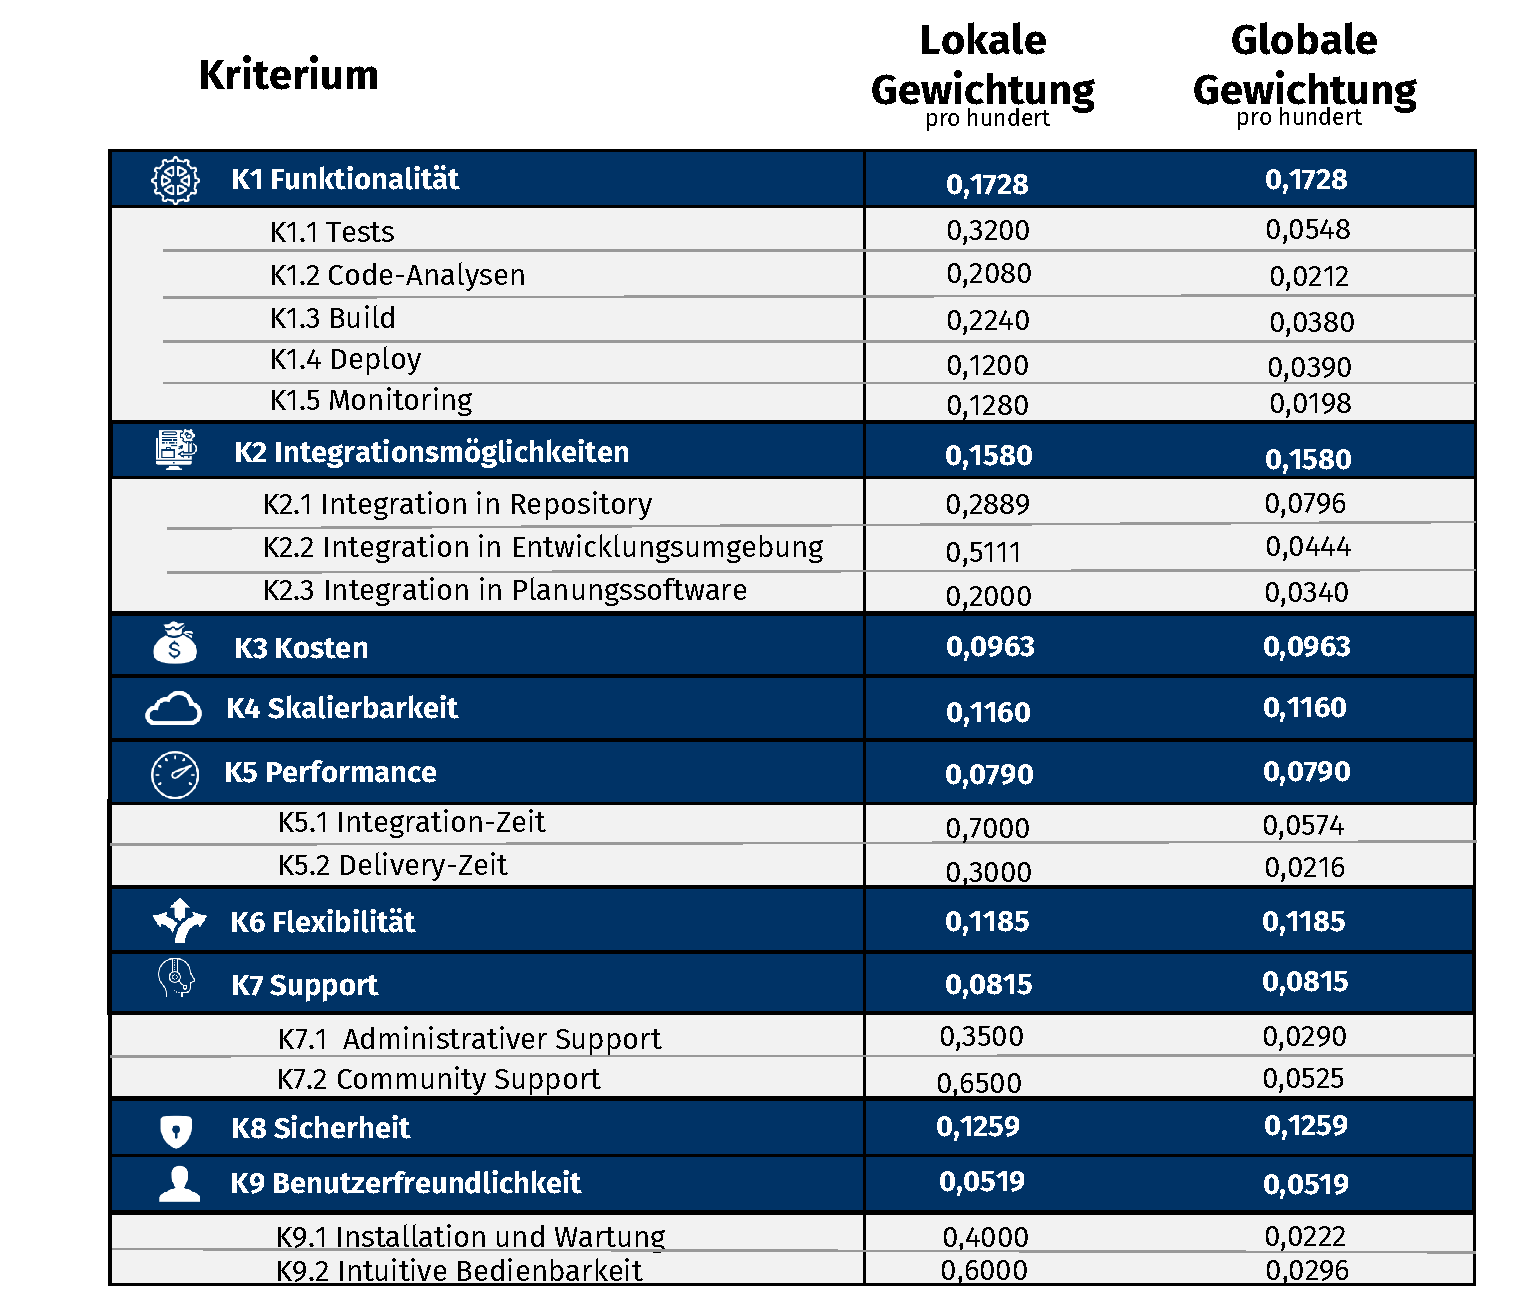
\includegraphics{AHP_G}}
		\caption[Gewichtungsfaktoren der AHP-Entscheidungskriterien]{Gewichtungsfaktoren der AHP-Entscheidungskriterien. Eigene Darstellung.}
		\label{fig:AHP_G}
	\end{figure}
\end{center}
\vspace*{-15mm}
Sowohl für den Fullstack- als auch die Test-Entwickler stellt die Unterstützung automatisierter Tests einen signifikanten Aspekt dar \cite[Z. 5 ff.]{BackendTestDeveloperSAPDTSIntegration.}. Da die Entwickler ein möglichst zeitnahes Feedback auf Code-Änderungen erhalten möchten, ist bei der Abwicklung dieser Tests insbesondere die Integration-Zeit, also das Intervall der Konsolidierung von Code-Änderungen in den Hauptzweig, essenziell \cite[Z. 23 ff.]{TestDeveloperSAPHyperspaceAdoption&Onboarding.b}. Für die Entwickler weniger wichtig ist in diesem Kontext die Delivery-Zeit, also die Dauer des Ausrollens von IT-Services auf das Produktionssystem. Dies ist darauf zurückführen, dass sich die Geschwindigkeit dieses Prozesses nicht unmittelbar auf die Produktivität  und Effizienz der Entwickler auswirkt. Kosten sind für die Entwickler ebenfalls von geringer Relevanz, da diese Experten während der operativen Tätigkeit kaum Berührungspunkte mit diesem Aspekt besitzen. Eine höhere Bedeutung hat für die Entwickler hingegen der Community-Support \cite[Z. 25 ff.]{FullStackEntwicklerSAPDTSIntegration.}. Dieser kann als Hilfestellung zur Implementation der Pipelines verwendet werden. Für den Product Manager sind die Integrationsmöglichkeiten ein wichtiger Aspekt. Gemäß empirischer Erkenntnisse ist die Wahl eines CI/CD-Tools, insbesondere von der Kompatibilität mit dem Repository abhängig \cite[Z. 5 ff.]{exp8}. Weniger wichtig sind für den Product Manager hingegen die Integrationsmöglichkeiten von Planungssoftware sowie Entwicklungsumgebung. Dies begründet der Experte damit, dass derartige Integrationen in der tatsächlichen Anwendungspraxis wenig Verwendung finden und die Wahl eines Pipeline-Tools daher durch diese Aspekte nicht tangiert wird. Weiterhin erachtet der Product Manager Sicherheit als einen essenziellen Aspekt. Da die Bereitstellung von Software zur Wertschöpfung beiträgt, können Unterbrechungen der CI/CD-Pipelines erhebliche Auswirkungen auf die Wettbewerbsfähigkeit besitzen. Überdies bieten CI/CD-Pipelines eine effektive Möglichkeit, um Schadsoftware in die Produktionssysteme einzuschleusen \cite[Z. 5 ff.]{exp8}. 

\subsection{Bewertung der Entscheidungsalternativen}
\label{sec:Bewertung}
Das erste zu bewertende Kriterium ist die \textbf{Funktionalität}. Sowohl für Jenkins als auch für Azure Pipelines wird die Programmbibliothek Project Piper verwendet. Mit dieser werden essenzielle, für die Bereitstellung von SAP-Technologien verwendete Pipeline-Funktionalitäten wie vorimplementierte Skripte, Test-Frameworks sowie Laufzeitumgebungen ausgeliefert. Daher erzielen beide CI/CD-Tools innerhalb der \textit{Funktionalität} weitgehend ähnliche Ergebnisse.\\ In Kriterium K1.1 (\textit{Tests}) wird die Unterstützung von Unit-, Integration-, E2E-, sowie Regression-Tests evaluiert. Mit Project Piper wird eine Test-Laufzeitumgebungen für Node zur Verfügung gestellt. Somit ist es möglich, Backend-Unit-Tests mittels Mocha und Jest auszuführen. Die Programmbibliothek unterstützt ebenfalls die für Frontend-Unit-Tests mittels Qunit und Frontend-Integration-Tests mittels OPA5 benötigte Laufzeitumgebung Karma. Darüber hinaus wird das für Backend-Integration-Tests benötigte Newmann-Tool bereitgestellt. Für E2E-Tests mittels WDI5 wird eine Webdriver-Laufzeitumgebung ausgeliefert \cite[Z. 66 ff.]{TestDeveloperSAPHyperspaceAdoption&Onboarding.}. Im Kontext der CEA stellt ebenfalls die Automatisierung von Regression-Tests einen essenziellen Faktor dar. Bei der Weiterentwicklung eines Microservice muss validiert werden, ob abhängige Dienste stets ordnungsgemäß funktionieren. Dafür wird mit Azure Pipelines und Jenkins ein Ressourcen-Trigger bereitgestellt \cite{Steved0x.20230410}\cite{.20230417}. Dieser gewährleistet ein automatisiertes Ausführen von Pipelines abhängiger Microservices. Dabei können sämtliche Tests der Anwendungen, welche den neuen Service konsumieren, erneut durchgeführt und validiert werden. In SAP CI/CD können alle Tests, mit Ausnahme der Backend-Integration-Tests mittels Newmann und der Regression-Tests ausgeführt werden. Dies stellt insbesondere für CEs einen erheblichen Nachteil dar. Diese sind aufgrund ihrer modularen IT-Architektur darauf angewiesen, dass einzelne Microservices reibungslos miteinander interagieren. Da ein implizites Validieren des Komponentenzusammenspiels ebenfalls über E2E-Tests abgewickelt wird, fällt dieser Nachteil jedoch weniger gewichtig aus. Aus diesem Grund wird eine Bewertung von drei Punkten für SAP CI/CD vergeben (Vorteile überwiegen Nachteilen). Für Azure Pipelines sowie Jenkins ist eine Bewertung von vier Punkten vorgesehen (ausschließlich Vorteile). In Kriterium K1.2 erfolgt eine Validierung der durch die Pipeline bereitgestellten \textit{Code-Analyse-Funktionalitäten}. Project Piper unterstützt statische Code-Analyse mittels Lint bzw. SonarQube, Sicherheitsüberprüfungen mittels Checkmarx und DASTER sowie Performance-Tests mittels JMeter \cite[Z. 40 ff.]{ProductManagerSAPHyperspaceSecurityTools.}. Mit dem SAP CI/CD-Tool sind ausschließlich statische Code-Analysen mittels Lint bzw. SonarQube möglich \cite[Z. 50 ff.]{ProductOwnerSAPBTPProd&Infra.}. Neben der fehlenden Unterstützung von Performance-Tests birgt insbesondere die Inkompatibilität von Sicherheits-Tools für eine CEA erhebliche Nachteile. Die CE-typische Verwendung von APIs zur Kommunikation zwischen einzelnen Microservices hat zur Folge, dass eine für unautorisierte Zugriffe begünstigte Angriffsfläche entsteht. Obwohl mögliche Sicherheitsbedenken auch durch Security-Experten manuell behoben werden könnten, ist dies für die von CEs angestrebte dynamische Reaktionsfähigkeit hinderlich. Zudem wird die Abwicklung von \textit{\ac{SAST}} mit Checkmarx bzw. \textit{\ac{DAST}} mit DASTER von der SAP als Produktqualitätsstandard vorgeschrieben \cite[Z. 37 ff.]{ProductManagerSAPHyperspaceSecurityTools.}. Somit kann das SAP CI/CD nicht von Kunden verwendet werden, welche sich an dem Sicherheitsstandard der SAP orientieren. Aus diesem Grund ergibt sich eine Bewertung von einem Punkt für SAP CI/CD (Nachteile überwiegen) und vier Punkten für Jenkins bzw. Azure Pipelines (ausschließlich Vorteile). In Kriterium K1.3 wird die \textit{Build-Funktionalität} der CI/CD-Tools evaluiert. Mit Project Piper wird dabei das für SAP UI5 sowie SAP CAP Node benötigte MTA-Build-Tool zur Verfügung gestellt. Weiterhin wird durch die Programmbibliothek ein Build-Tool für Docker-Container sowie eine Funktion zur Einbindung des von der SAP bereitgestellten Artefakt-Repositorys Artefactory bereitgestellt \cite{.20230406}. SAP CI/CD unterstützt kein Docker-Workflow sowie Artefakt-Repository \cite{.20230406b}. Besonders gewichtig ist dabei die fehlende Unterstützung des Artefakt-Repositories. Artefakt-Repositories spielen für CEs eine essenzielle Rolle bei der Durchführung von Rollbacks. Bei dem Auftreten von Fehlern eines Services kann zu einer früheren im Artefakt-Repository abgelegten Version zurückgekehrt werden. Somit wird das Risiko von Ausfällen und Unterbrechungen im Geschäftsbetrieb minimiert. Da SAP CI/CD dennoch das für SAP CAP Node und SAP UI5 benötigte MTA-Build-Tool bereitstellt und somit den minimal erforderlichen Satz an benötigter Build-Funktionalität unterstützt, wird eine Bewertung von zwei Punkten veranschlagt (Nachteile und Vorteile gleichgewichtig). Für Azure Pipelines sowie Jenkins wird eine Bewertung von 4 Punkten vergeben (ausschließlich Vorteile). In Kriterium K1.4 erfolgt die Evaluierung der \textit{Deploy- und Release-Funktionalitäten}. Dabei herrscht bei SAP CI/CD, Azure Pipelines sowie Jenkins Feature-Parität. Ein erheblicher Mehrwert besteht insbesondere darin, dass alle zu untersuchende CI-CD-Lösungen eine Bereitstellung in das SAP CTM unterstützen (s. Abb. \ref{fig:CTM}).
Durch den Einsatz dieses Tools lässt sich die Bereitstellung von Software innerhalb komplexer ERP-Systemlandschaften optimieren. Ein Unternehmen könnte etwa separate Systeme für das Entwickeln (\textit{DEV}), Testen (\textit{TEST}) sowie für die Produktionsumgebung (\textit{PROD}) besitzen (s. Abb \ref{fig:CTM}). Während die Verantwortung der Entwickler dabei auf die ordnungsgemäße Bereitstellung der Funktionalitäten in das DEV-System beschränkt ist, werden nachfolgende Schritte von dem Betriebsteam über das SAP CTM verwaltet. Über dieses System können dabei vielfältige Release-Konfigurationen, wie z.B. eine zeitplangesteuerte Bereitstellung vorgenommen werden. Des Weiteren ermöglicht das SAP CTM die Definition von Abhängigkeiten verschiedener Services. Experte 2 merkt an, dass dies insbesondere für eine CEA von hoher Bedeutung ist \cite[Z. 67 ff.]{ProductManagerSAPHyperspaceCICD.}. Im Falle einer API-Änderung bestimmter Microservices besteht die Möglichkeit, dass in konsumierenden Diensten entsprechend Fehler auftreten. Mittels des SAP CTMs kann dabei jedoch reguliert werden, dass die neue Version eines Microservices erst nach Anpassung der abhängigen Dienste in das Produktivsystem eingeführt wird.
\begin{center}
	\begin{figure}[H]
		\centering
		\scalebox{0.3}{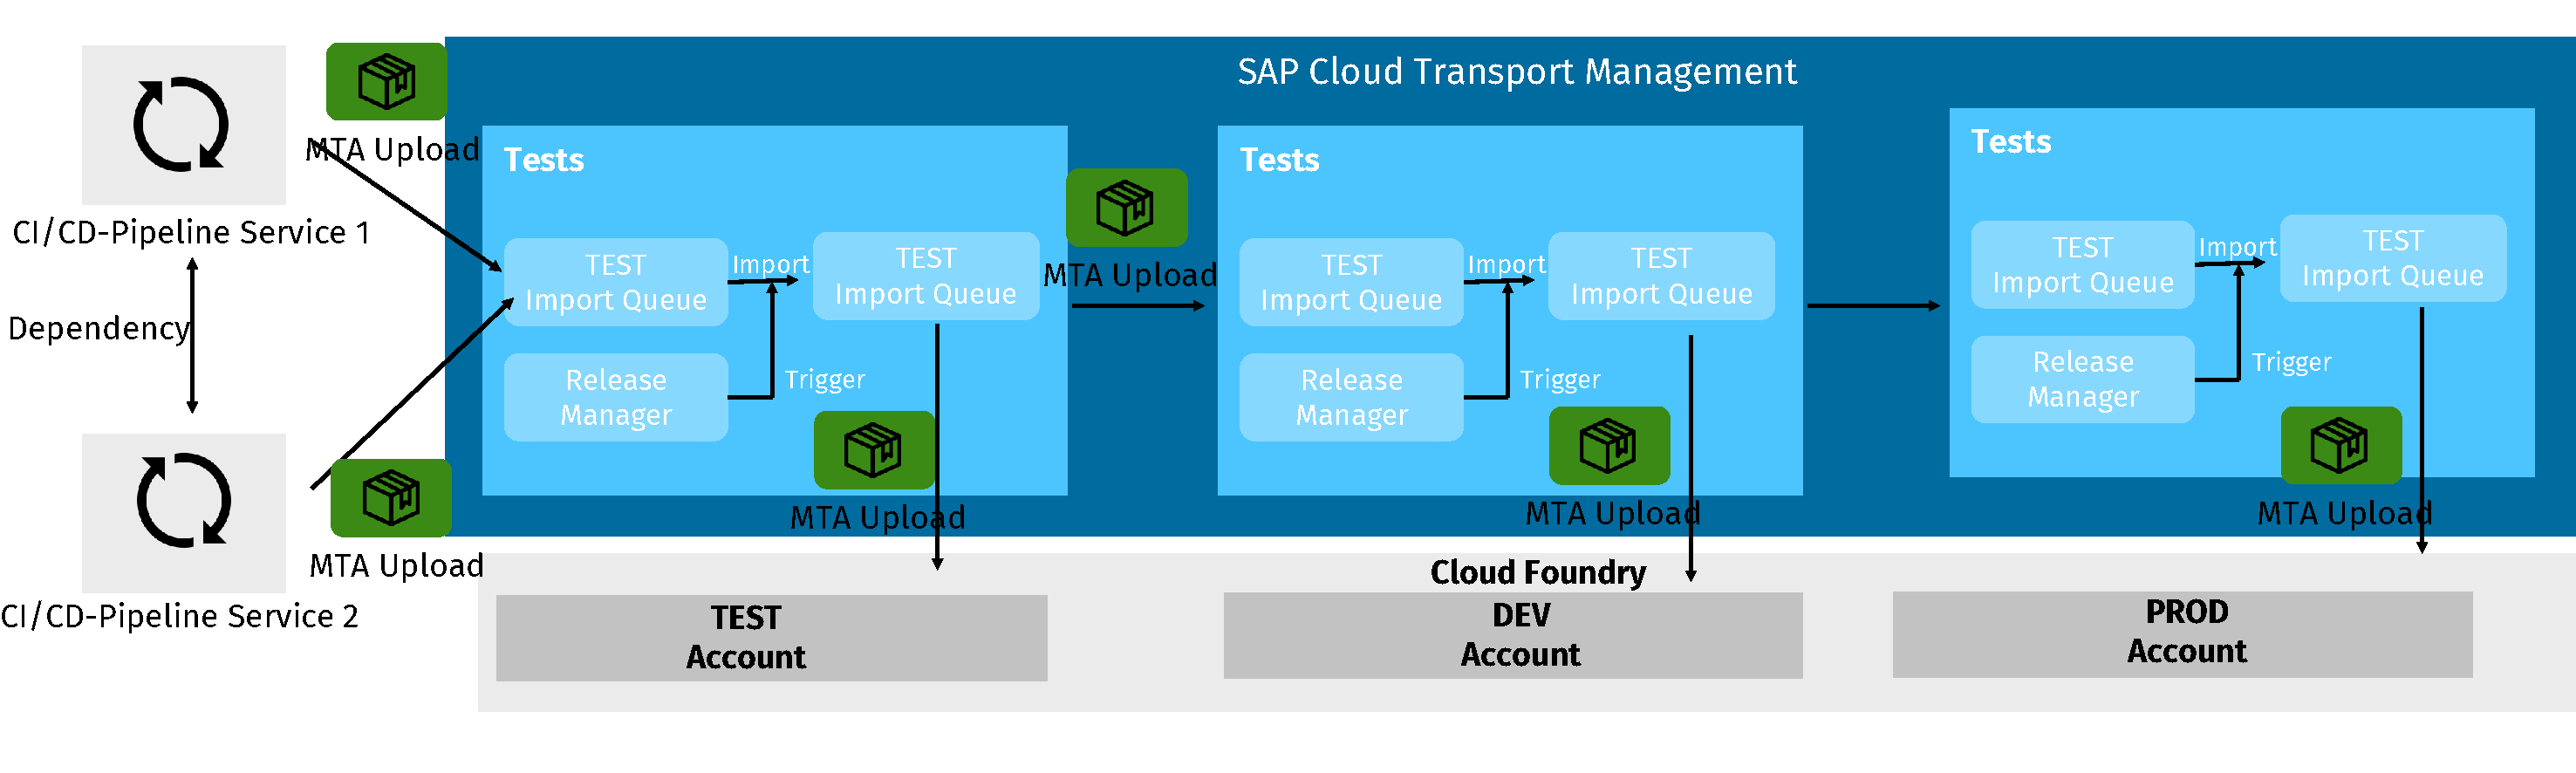
\includegraphics{CTM}}
		\caption[SAP Cloud Transport Management]{SAP Cloud Transport Management. In Anlehnung an Stevens \cite{.20230327}.}
		\label{fig:CTM}
	\end{figure}
\end{center}
\vspace*{-15mm}
Weiterhin wird von den Pipelines neben dem Multi-Cloud- ebenfalls das Blue/Green-Deployment unterstützt \cite{.20230406c}. Da das Blue/Green-Deployment eine hohe Flexibilität und Agilität im Bereitstellungsprozess gewährleistet, stellt dieses für CEs einen hohen Mehrwert dar. Mit dieser Deployment-Strategie wird neben der zu installierenden neuen Version ebenfalls die stabile Anwendung betrieben. Bei erfolgreicher Inbetriebnahme kann der Datenverkehr unmittelbar auf die neue Instanz umgeleitet werden, wobei Unterbrechungszeiten vermieden werden können. Dies spielt insbesondere im Kontext von Composable-ERP-Systemen, in welchem kritische Prozesse, wie die Überwachung von Zahlungsströmen abgewickelt werden, eine bedeutende Rolle. Während alle CI/CD-Tools eine Cloud-Foundry-, CTM-, Multi-Cloud- sowie Blue/Green-Bereitstellung unterstützen, ist Canary- sowie Shadow-Deployment nicht möglich. Da diese jedoch ausschließlich ergänzende Zusatzfunktionalitäten und keine essenziell benötigten Werkzeuge darstellen, wird für Azure Pipelines, Jenkins sowie SAP CI/CD eine Bewertung von 3 Punkten vergeben (Vorteile überwiegen). In Kriterium K1.5 wird die \textit{Monitoring-Funktionalität} der Pipelines untersucht. Mit Project Piper können im CI/CD-Prozess generierte Logs unmittelbar an das Monitoring-Dashboard Splunk übermittelt werden \cite[Z. 74 ff.]{ProductManagerSAPHyperspaceCICD.}. Open-Soruce-Tools wie das Kibana-Dashboard lassen sich dabei ebenfalls mit Jenkins bzw. Azure Pipelines verknüpfen. Während Kibana unmittelbar als Azure-SaaS-Tool verfügbar ist, benötigt das Aufsetzen auf Jenkins einen deutlich höheren Aufwand (s. Abb. \ref{fig:kibana}). So müssen auf der Jenkins-Plattform Tools zum Versenden (Beats), Transformieren (Logstash) bzw. zum Speichern (Elasitcsearch) der Pipeline-Logs manuell aufgesetzt werden. Um die Pipeline-Metriken letztlich auf dem Dashboard zu visualisieren, müssen die Logs über APIs an eine extern gehostete Kibana-Instanz übermittelt werden \cite{Atta.20201012}. Der SAP CI/CD-Service unterstützt ausschließlich eine Protokollierung der Build-Logs einzelner Pipelines.
\begin{center}
	\begin{figure}[H]
		\centering
		\scalebox{0.3}{\includegraphics{kibana}}
		\caption[Pipeline-Monitoring mit Kibana und Jenkins]{Pipeline-Monitoring mit Kibana und Jenkins. In Anlehnung an Atta \cite{Atta.20201012}}
		\label{fig:kibana}
	\end{figure}
\end{center}
\vspace*{-15mm}
 Für Experte 2 stellt die Inkompatibilität von Monitoring-Dashboards insbesondere in einer Microservice-Architektur einen erheblichen Nachteil dar. So sind die zentralen Dashboards bei aus komplexen Diensten bestehenden Systemarchitekturen häufig die einzige Möglichkeit CI/CD-Prozesse nachhaltig zu überwachen \cite[Z. 38 ff.]{ProductManagerSAPHyperspaceCICD.}. Während für Azure Pipelines vier Punkte vergeben werden (ausschließlich Vorteile), erhält Jenkins aufgrund des hohen Einrichtungsaufwands für das Kibana-Dashboard eine Bewertung von drei Punkten (Vorteile überwiegen Nachteilen). Für SAP CI/CD wird aufgrund der fehlenden Unterstützung von Monitoring-Dasboards ausschließlich ein Punkt vergeben (Nachteile überwiegen Vorteilen).\\ In Kriterium K2 werden die \textbf{Integrationsmöglichkeiten} der Pipelines evaluiert. Alle drei Pipelines unterstützen dabei eine Integration der Repositories GitHub, BitBucket und GitLab. Für Jenkins und SAP CI/CD müssen dafür jedoch manuell in den entsprechenden Repositories Webhooks aufgesetzt werden. Ein Webhook ist eine API, welche Anfragen zum Auslösen eines CI/CD-Workflows an die Pipeline übermittelt. Diese Webhook-Anfragen können bei einer Vielzahl von Events, einschließlich dem \textit{Pushen} von Codeänderungen oder dem Eröffnen von \textit{Pull-Requests}, ausgelöst werden. SAP CI/CD unterstützt dabei keine Pull-Request-Webhooks. Dies birgt im Entwicklungsprozess erhebliche Nachteile. Eine Pull-Request-Pipeline gewä\-hrleistet, dass Entwicklungen eines Feature-Branches erst nach erfolgreicher Abwicklung aller Tests in den Hauptzweig integriert werden \cite[Z. 27 ff.]{ProductOwnerSAPBTPProd&Infra.}. Ohne diese Funktionalität muss die Pipeline bei Erstellung eines Pull-Requests stets manuell gestartet und überprüft werden, was zur Beeinträchtigung der Zusammenarbeit in Teams führt. Für Azure Pipelines wird eine Bewertung von vier Punkten vergeben (ausschließlich Vorteile). Jenkins erhält aufgrund der Notwendigkeit einer manuellen Webhook-Konfiguration drei Punkte (Vorteile überwiegen). Da SAP CI/CD darüber hinaus keine Pull-Request-Pipelines unterstützt und diese laut Experte 1 in einigen Entwicklungsabteilungen gängige Praxis darstellen, wird eine Bewertung von zwei Punkten vergeben (Vorteile und Nachteile gleichgewichtig) \cite[Z. 27 ff.]{ProductOwnerSAPBTPProd&Infra.}. In Jenkins sowie Azure Pipelines lassen sich die Entwicklungsumgebungen Microsoft Visual Studio Code sowie Eclipse integrieren (\textit{Integrationsmöglichkeiten von Repositories (Kriterium K2.2)}). Das SAP CI/CD unterstützt keine Integration der zu evaluierenden Entwicklungsumgebungen \cite[Z. 94 ff.]{ProductOwnerSAPBTPProd&Infra.}. Somit ist es Entwicklern nicht möglich, die CI-Pipeline unmittelbar aus der Entwicklungsumgebung zu starten. Da sowohl für Azure Pipelines als auch Jenkins ausschließlich zwei der drei zu evaluierenden Entwicklungsumgebung unterstützt werden, wird eine Bewertung von drei Punkten vergeben (Vorteile überwiegen Nachteilen). SAP CI/CD wird aufgrund der fehlenden Integrationsmöglichkeiten mit null Punkten bewertet (ausschließlich Nachteile). Sowohl mit Azure Pipelines als auch Jenkins lassen sich Planungs-Tools wie Jira integrieren (\textit{Integrationsmöglichkeiten von Planungssoftware (Kriterium K2.2)}). Für SAP CI/CD besteht diese Integrationsmöglichkeit nicht \cite[Z. 101 ff.]{TestDeveloperSAPHyperspaceAdoption&Onboarding.}. Demnach ist es Projektmanagern nicht möglich, den Build-Status verschiedener Backlog-Items zu überwachen. Aus diesem Grund ergibt sich eine Bewertung von vier Punkten für Azure Pipelines sowie Jenkins bzw. null Punkte für das SAP CI/CD.\\ In Kriterium K3 werden die \textbf{Kosten} der CI/CD-Tools evaluiert. Für SAP CI/CD werden Gebühren von einem Euro pro Build-Stunde fällig \cite[Z. 107 ff.]{ProductOwnerSAPBTPProd&Infra.}. Azure Pipelines berechnet hingegen unabhängig von der Nutzungszeit 40 Euro pro Pipeline \cite{.20230410}. In den genannten Preisen werden Kosten für die IT-Infrastruktur, Installation, Wartung sowie Support berücksichtigt. Zwar fallen für die Jenkins-Pipeline keine Lizenzgebühren an, jedoch müssen im Gegensatz zu den SaaS-Tools weitere Kostenpositionen beachtet werden. Da Jenkins in einem On-Premise-Modell betrieben wird, fallen zunächst Investitionskosten für Hardware an. Weiterhin müssen für den On-Premise-Server laufende Betriebskosten, wie Ausgaben für Energie, Reparaturleistungen und Personal zur Wartung der IT-Infrastruktur berücksichtigt werden. Untersuchungsergebnisse des IT-Beratungshauses ExecuTech zeigen, dass On-Premise-Systeme aufgrund hoher Investitionskosten insbesondere bei einer kurzfristigen Betrachtung teurer sind \cite{Executech.20230308}. Eine langfristige Perspektive führt jedoch zu einem anderen Ergebnis. Da die laufenden Betriebskosten für On-Premise-Systeme häufig geringer als die SaaS-Gebühren sind, können diese auf lange Sicht kosteneffektiver werden. CEs sind jedoch darauf ausgerichtet, flexibel und agil zu agieren, um auf sich ändernde Geschäftsanforderungen reagieren zu können. Somit müssen diese in der Lage sein, Systeme schnell auf- und abzubauen. Dies würde im On-Premise-Modell kontinuierliche Investitionskosten verursachen, wobei SaaS ebenfalls auf längere Sicht die günstigere Alternative bleibt. Aus diesem Grund wird für die SaaS-Systeme Azure Pipelines und SAP CI/CD eine Bewertung von drei Punkten bzw. für Jenkins einen Punkt vergeben (Nachteile überwiegen Vorteilen).\\ In Kriterium K4 wird die \textbf{Skalierbarkeit} der Tools evaluiert. Mit Azure Pipelines lässt sich die CI/CD-Pipeline eines Microservices horizontal skalieren. Um parallele Builds auszuführen, werden hierbei mehrere \textit{Microsoft-hosted Agents} aktiviert. Ein Microsoft-hosted Agent ist eine von Azure verwaltete virtuelle Maschine, welche eine vorkonfigurierte Build- und Testumgebung bereitstellt \cite{Steved0x.20230410b}. Eine vertikale Skalierung kann dabei durch das Zuweisen zusätzlicher Ressourcen zu einem Microsoft-hosted Agent erreicht werden. Während eine horizontale Skalierung ebenfalls über das Hinzufügen zusätzlicher Agents ermöglicht wird, ist eine vertikale Skalierung aufgrund architektonischer Limitationen bei Jenkins nur begrenzt möglich \cite{.20230410b}. So müssen in das bestehende System zusätzliche Hardware-Ressourcen integriert werden. Das bedeutet, dass die vertikale Skalierbarkeit auf die physischen Einschränkungen eines Servers begrenzt ist. Während horizontale Skalierung von SAP CI/CD unterstützt wird, ist eine vertikale Skalierung nicht realisierbar. Die vertikale Skalierbarkeit von CI/CD-Pipelines spielt jedoch insbesondere in einem volatilen Geschäftsumfeld eine signifikante Rolle. Als eines der größten CEs stellt der Streaminganbieter Netflix über 1000 Microservices bereit. Angesichts der Notwendigkeit, für jeden Microservice mindestens eine CI/CD-Pipeline bereitzustellen, würde ein nicht skalierbares Pipeline-System eine umfangreiche IT-Infrastruktur erfordern. Netflix setzt aus diesem Grund auf eine vertikal-skalierbare Container-Orchestrierungstechnologie \cite{Blog.20170419}\cite{CloudZero.20230419}. Mit dieser werden zur Laufzeit Pipelines in Docker-Container bereitgestellt, welche je nach Bedarf auf- oder abgebaut bzw. skaliert werden können. So wird Azure Pipelines mit vier Punkten (ausschließlich Vorteile) und Jenkins sowie SAP CI/CD mit einem Punkt bewertet (Nachteile überwiegen Vorteilen).\\ In Kriterium K5 wird die \textbf{Performance} der Pipelines evaluiert. Zur Durchführung dieser Analyse wird ein speziell für die Arbeit entwickelter Prototyp einer CEA verwendet. Dieser besteht aus drei Microservices, welche jeweils ein Frontend (SAP UI5), eine Service-API (SAP CAP Node) sowie eine Datenbank (SAP HANA) besitzen (s. Abb. \ref{fig:Szenario}).
 \begin{center}
	\begin{figure}[H]
		\centering
		\scalebox{0.3}{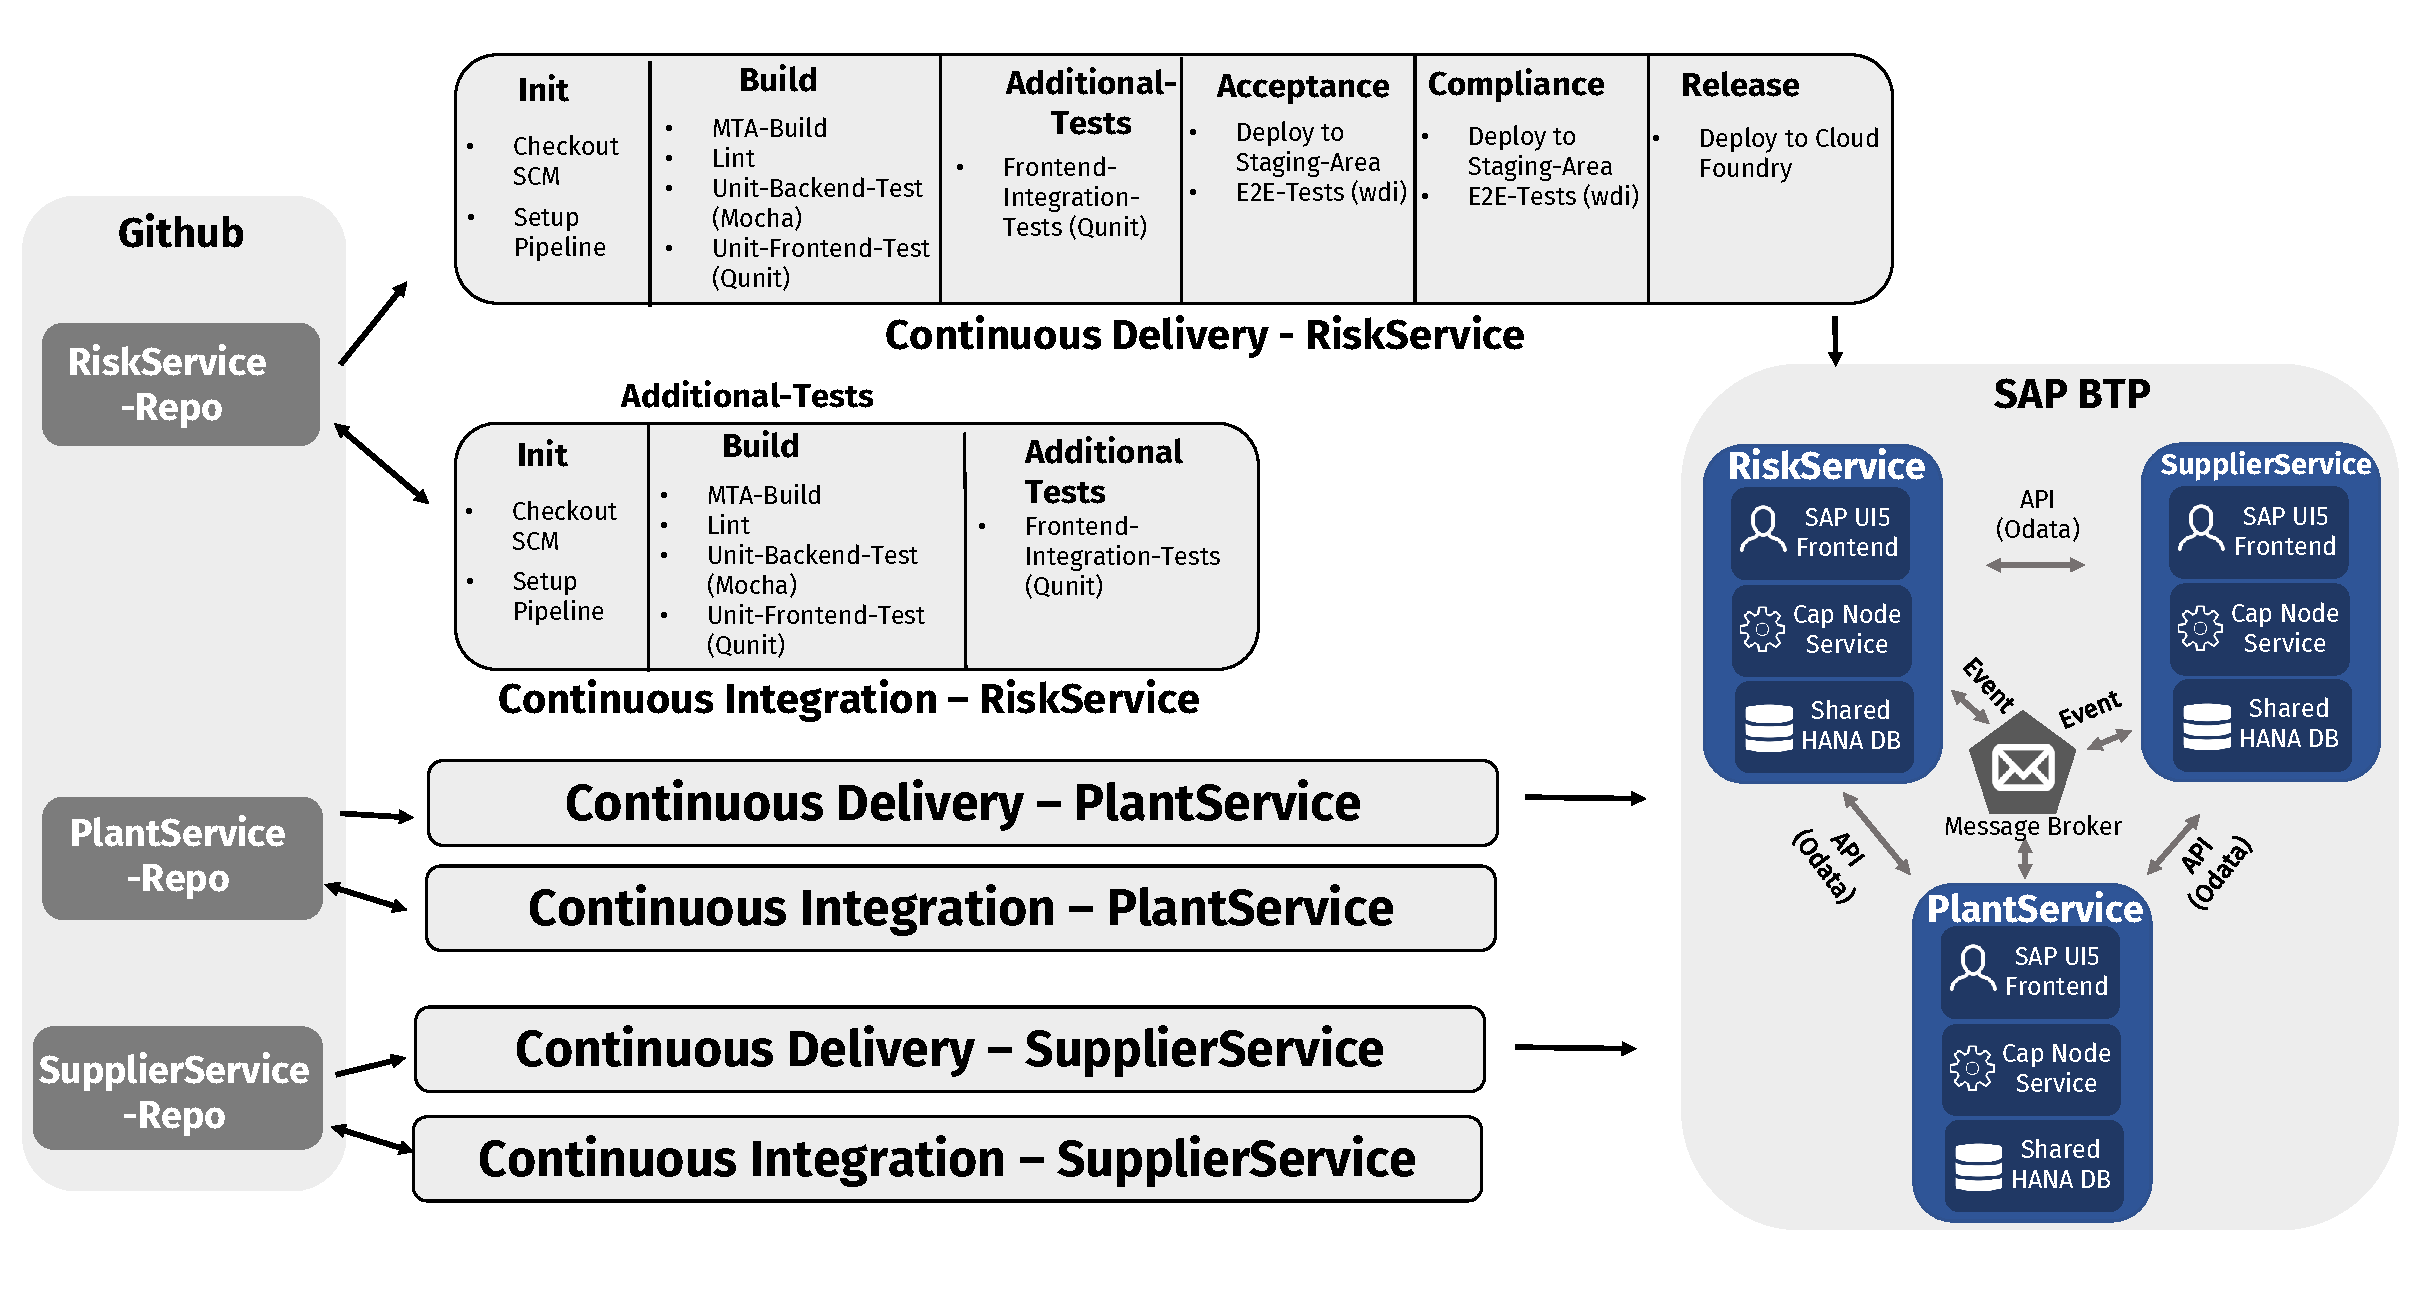
\includegraphics{Szenario}}
		\caption[CEA-Szenario für Performance-Tests]{CEA-Szenario für Performance-Tests. Eigene Darstellung.}
		\label{fig:Szenario}
	\end{figure}
\end{center}
\vspace*{-15mm}
 Des Weiteren ist mit den zu untersuchenden Tools für jeden Microservice eine eigene CI- sowie CD-Pipeline implementiert. Die CI-Pipeline besteht hierbei aus einem MTA-Build, statischen Lint-Code-Analysen, Backend-Unit-Tests, Frontend-Unit- sowie -Integration-Tests. Die CD-Pipeline erweitert den CI-Prozess um Sonar-Qube-Code-Analysen, End-To-End-Tests sowie einem Schritt zur Bereitstellung der Anwendung auf der SAP BTP. Im Vergleich zu den anderen zu evaluierenden Tools weist das SAP CI/CD den geringsten Funktionsumfang auf. Um eine bessere Vergleichbarkeit zu gewährleisten, ist der Aufbau der anderen Pipelines strukturell an den Funktionsumfang dieses Tools angepasst. So sind etwa für keine der Pipelines Integration-Tests, sowie Security-Scans implementiert. Für jedes zu untersuchende CI/CD-Tool wird dabei die Durchlaufzeit der Pipelines aller drei Microservices in Sekunden gemessen. Anschließend werden die Einzelmessungen der Services aggregiert, um für jedes zu evaluierende CI/CD-Tool eine Integration- sowie Delivery-Zeit zu erhalten (s. Anhang \ref{fig:JP_Risk}). Die Ergebnisse der Tests zeigen, dass für den vollständigen Durchlauf der CI-Prozesse aller Microservices für Azure Pipelines 600 Sekunden, Jenkins 1134 Sekunden und SAP CI/CD 1243 Sekunden benötigt werden (s. Tab. \ref{tab:Performance}). Unter der in Kapitel \ref{sec:Metriken} spezifizierten Metrik ergibt sich im \textit{Kriterium K5.1} eine Bewertung von vier Punkten für Azure Pipelines (bester Zeitwert). Für Jenkins sowie SAP CI/CD werden hingegen null Punkte vergeben (75 Prozent oder mehr über dem besten Zeitwert).  Für die vollständige Abwicklung des CD-Prozesses werden für Azure Pipelines 2194 Sekunden, Jenkins 3409 Sekunden und SAP CI/CD 3801 Sekunden benötigt. Daraus resultiert im \textit{Kriterium K5.2} eine Bewertung von vier Punkten für Azure Pipelines (bester Zeitwert) und einem Punkt für Jenkins bzw. SAP CI/CD (50 Prozent bis 75 Prozent über dem besten Zeitwert). Die überdurchschnittliche Leistungsfähigkeit von Azure Pipelines lässt sich auf verschiedene Faktoren zurückführen. Zum einen erfolgt der Betrieb der Pipeline-Systeme unter Einsatz modernster Hardwaretechnologien. Darüber hinaus werden durch Azure Pipelines ebenfalls Mechanismen wie \textit{Parallel Builds} und \textit{Caching} im Standard unterstützt. Während bei Parallel-Builds das Ausführen gleichzeitiger Pipeline-Schritte ermöglicht wird, gewährleistet Caching, dass während des CI/CD-Workflows heruntergeladene Ressourcen für zukünftige Pipeline-Durchläufe zwischengespeichert werden. Dies führt zur erheblichen Beschleunigung der Integration- bzw. Delivery-Prozesse.
 \begin{center}
	\begin{table}[H]
		\centering
		\scalebox{0.3}{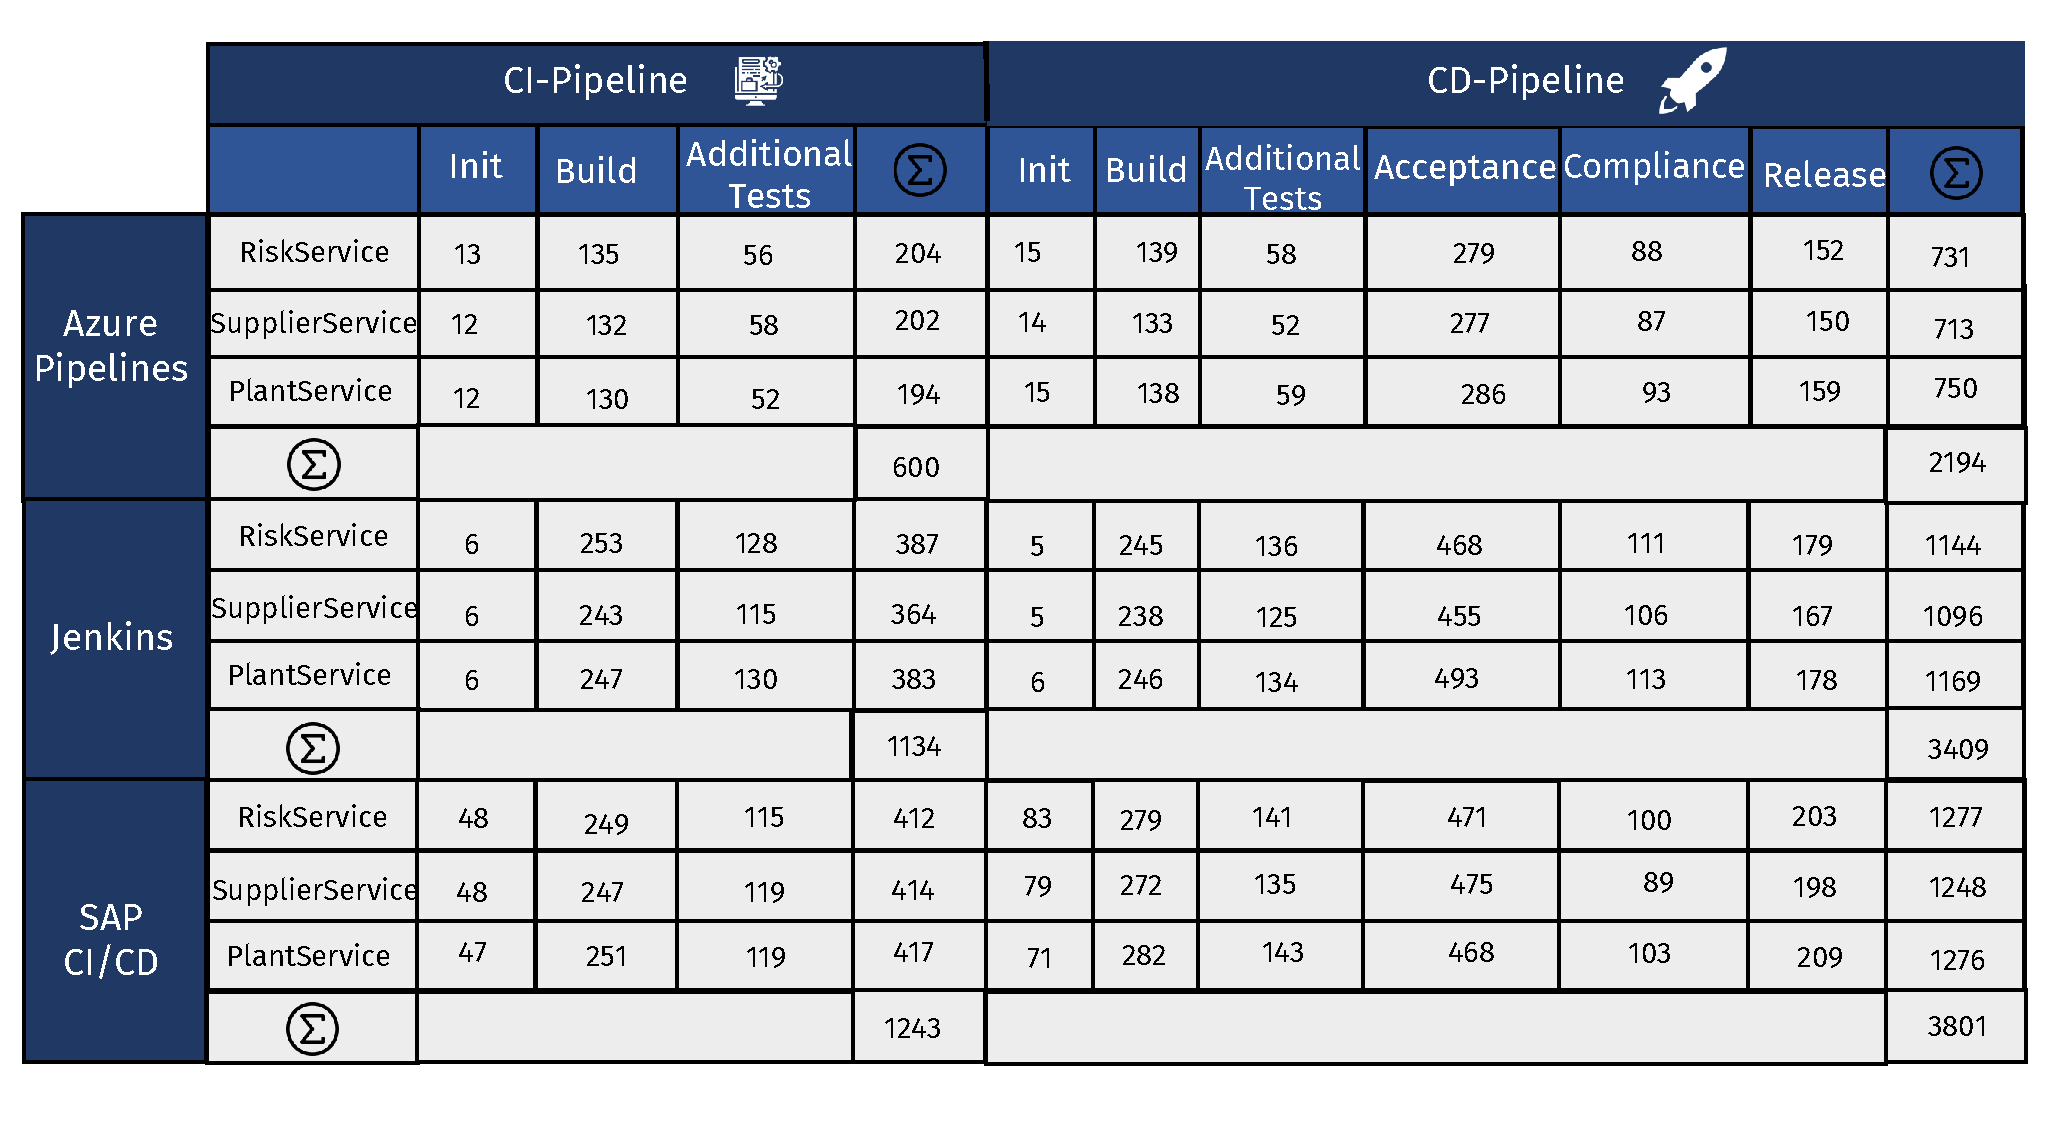
\includegraphics{Performance}}
		\caption[Integration- und Delivery-Zeit in Sekunden]{Integration- und Delivery-Zeit in Sekunden. Eigene Darstellung.}
		\label{tab:Performance}
	\end{table}
\end{center}
\vspace*{-15mm}
 Die Ergebnisse dieses Performance-Tests sind jedoch differenziert zu betrachten. Die Überprüfungen wurden ausschließlich anhand von Prototypen mit einem geringem Umfang an Programmcode durchgeführt. Somit ist zu berücksichtigen, dass die Ergebnisse bei umfangreicheren Produktivprojekten abweichen können. Angesichts des erheblichen zeitlichen Abstands lässt sich annehmen, dass Azure Pipelines nach wie vor die beste Performance besitzt. Zudem ist zu beachten, dass Jenkins On-Premise betrieben wird und somit bei einer divergierenden Hardware auch unterschiedliche Leistungsergebnisse erzielt werden können.\\ In Kriterium K6 wird die \textbf{Flexibilität} der Services evaluiert. Sowohl mit Azure als auch Jenkins lassen sich die mit der Programmbibliothek Project Piper bereitgestellten CI/CD-Schritte (z.B. Build, Test etc.) frei nach Bedarf kombinieren und konfigurieren. SAP CI/CD besitzt dabei maßgebliche Einschränkungen. Hierbei werden Anzahl, Reihenfolge sowie Konfiguration der Schritte von dem Service vorgeschrieben. Somit ist keine flexible Implementierung der Pipelines möglich. Laut Experte 5, stellt Technologieoffenheit einen fundamentalen Wert in einer CEA dar \cite[Z. 13 ff.]{SoftwareArchitektSAPDTSIntegration.}. So sollte die CI/CD-Pipeline verschiedene Programmier-Frameworks, Test-Frameworks und Cloud-Plattformen unterstützen. Damit werden bei Jenkins mehr als 1800 Plug-ins bereitgestellt, mit welchen über den Standard hinausgehende Funktionalitäten integriert werden können \cite{.20230410c}. Während mit Azure Pipelines 1400 Plug-ins bereitgestellt werden, besteht diese Möglichkeit bei SAP CI/CD nicht \cite{.20230410d}. Weiterhin sollten die CI/CD-Tools, um schnell neue Pipelines implementieren zu können, einen flexiblen modularen Aufbau ermöglichen. Bei Azure Pipelines und Jenkins können Shared-Librarys, wie Project Piper verwendet werden (s. Abb. \ref{fig:Modular}).
 \begin{center}
	\begin{figure}[H]
		\centering
		\scalebox{0.6}{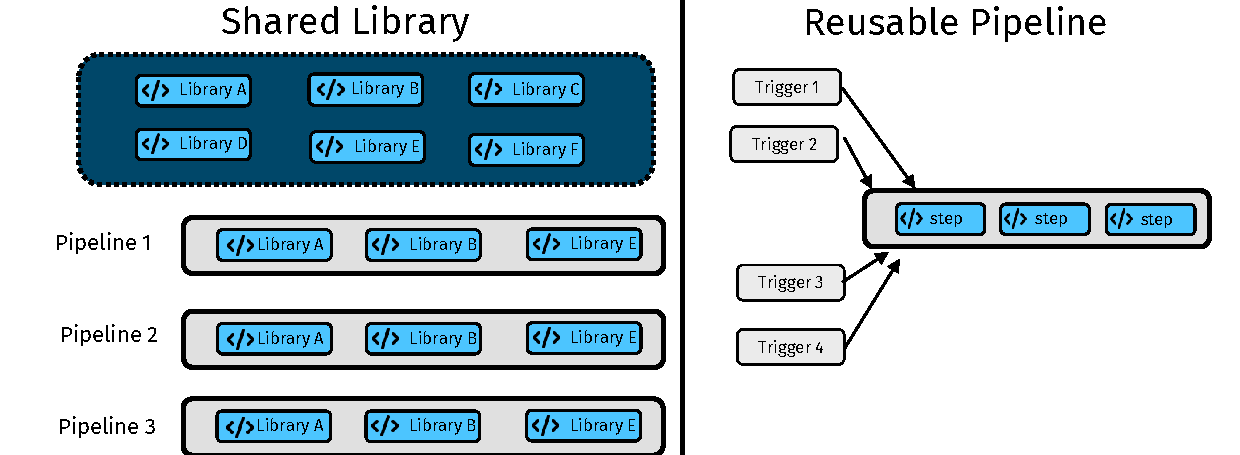
\includegraphics{Modular}}
		\caption[Modularer Aufbau einer CI/CD-Pipeline]{Modularer Aufbau einer CI/CD-Pipeline. In Anlehnung an Codefresh \cite{.20230402}.}
		\label{fig:Modular}
	\end{figure}
\end{center}
\vspace*{-15mm}
 Damit ist es möglich vorimplementierte Funktionalitäten, wie z.B. standardisierte Build, Deploy oder Test-Schritte in einer gemeinsamen Bibliothek zu konsolidieren. Eine weitere Möglichkeit, um die Komplexität der Bereitstellung zu reduzieren, besteht in der Wiederverwendung ganzer Pipelines. Dieses Konzept wird verwendet, wenn sämtliche Microservices einen homogenen Bereitstellungszyklus durchlaufen. Durch die Wiederverwendung ganzer Pipelines kann somit sichergestellt werden, dass diese auf analoge Weise kompiliert, verpackt und bereitgestellt werden. Bei Jenkins und Azure lässt sich dies durch die Einbindung mehrerer Repositories in eine Pipeline realisieren. Das SAP CI/CD stellt ebenfalls eine Shared-Library bereit. So werden die templatebasierten Schritte als standardisierte Elemente einer CI/CD-Pipeline ausgeliefert. Im Gegensatz zu Azure Pipelines und Jenkins gewährleistet dieses Tool jedoch lediglich die Integration der von dem SAP CI/CD bereitgestellten Bibliothek, wobei die Möglichkeit der Einbindung benutzerdefinierter Librarys nicht besteht. Die Wiederverwendung ganzer Pipelines für unterschiedliche Microservices ist ebenfalls nicht möglich.
Während der SAP CI/CD-Service das Shared-Library-Konzept im begrenzten Maße  unterstützt, ist eine flexible Implementierung der Pipelines, die Einbindung von Plug-ins, sowie die Wiederverwendung von CI/CD-Pipelines nicht möglich. Deshalb wird für den SAP CI/CD-Service eine Bewertung von einem Punkt vergeben (Nachteile überwiegen Vorteilen). Da Jenkins und Azure Pipelines bei den zu untersuchenden Entscheidungskriterien nur Vorteile bieten, werden jeweils vier Punkte vergeben.\\ In Kriterium K8 wird der \textbf{Support} der CI/CD-Tools evaluiert. Azure Pipelines stellt einen umfangreichen \textit{administrativen Support} bereit (Kriterium K7.1). Dazu gehört der für Kunden bereitgestellte Premium-Support \cite{.20230410e}. Bei diesem handelt es sich um eine kostenpflichtige Leistung, welche den Kunden unmittelbaren Zugang zu technischem Support und Beratung gewährt. Die Unterstützung beinhaltet Installation bzw. Konfiguration von Pipelines sowie der Integration einer vorhanden CI/CD-Toolchain (Tests, Repositories etc.) einschließlich der Optimierung der Pipeline-Performance. Zudem wird über das Azure-Support-Center ein kostenfreies Support-Ticket-System für Nicht-Premium-Nutzer angeboten. Diese Kanäle können verwendet werden, um allgemeine technische Probleme des CI/CD-Services zu melden. Weiterhin wird von Azure eine umfangreiche Dokumentation sowie Schulungsmaterialien, einschließlich Online-Tutorials, Videos und Webinare bereitgestellt. Der SAP CI/CD-Service stellt über den Drittanbieter Service Now ebenfalls ein kostenfreies Ticket-System zur Verfügung. Für spezifische Fragestellungen und individuelle Unterstützung besteht für Kunden die Möglichkeit, sich an die technische Beratung der SAP wenden \cite[Z. 113 ff.]{ProductOwnerSAPBTPProd&Infra.}. Wie auch bei Azure Pipelines stehen für SAP CI/CD Schulungs- und Dokumentationsunterlagen zur Verfügung. Für Jenkins sind diese Informationsmaterialien ebenfalls vorhanden, jedoch ist der administrative Support aufgrund des Open-Source-Charakters im Vergleich zu den anderen Lösungen begrenzt. Dies ist insbesondere auf das Fehlen eines unmittelbaren Supports durch einen Service-Anbieter zurückzuführen. Ebenso spiegelt sich dieser Aspekt in der Verfügbarkeit von Updates wider. Viele der Funktionalitäten von Jenkins werden über Open-Source-Plug-ins bereitgestellt. Experte 6 merkt an, dass hierbei stets das Risiko besteht, dass die Wartung einzelner Plug-ins in Zukunft vernachlässigt werden könnte \cite[29 ff.]{FullStackEntwicklerSAPDTSIntegration.}. Aus den aufgeführten Aspekten ergibt sich eine Bewertung von vier Punkten für Azure Pipelines sowie dem SAP CI/CD-Service (ausschließlich Vorteile). Für Jenkins wird eine Bewertung von einem Punkt vergeben (Nachteile überwiegen). Aufgrund des Open-Source-Charakters ist für die Jenkins-Pipeline ein umfassender \textit{Community-Support} vorhanden (\textit{Kriterium K7.2}). Jenkins ist dabei auf zahlreichen hochfrequentierten Foren vertreten. So wurden auf Stack-Overflow bereits 112.000 Posts zur Jenkins-Pipeline veröffentlicht \cite{StackOverflow.20230403d}. Dadurch wird den Anwendern Zugang zu einer breiten Palette an Ressourcen ermöglicht. Experte 4 merkt an, dass insbesondere die Gamifizierung dieser Plattformen zu einer schnellen und effektiven Unterstützung durch Spezialisten beiträgt. Auch Azure Pipelines sowie der SAP CI/CD sind ebenfalls auf öffentlichen Community-Foren vertreten, jedoch ist der dort publizierte Inhalt im Vergleich zu Jenkins signifikant geringer. Das liegt an der Tatsache, dass die genannten Pipelines als SaaS-Lösungen konzipiert sind und somit weniger Raum für fragebedürftige Anpassungen besteht. So sind für Azure Pipelines 25.000 Post und für SAP CI/CD lediglich 26 Einträge auf Stack-Overflow veröffentlicht \cite{StackOverflow.20230403b}\cite{StackOverflow.20230403c}. Gemäß der in Kapitel \ref{sec:Metriken} festgelegten Metrik wird eine Bewertung von vier Punkten für Jenkins (höchste Blog-Post-Anzahl) bzw. von null Punkten für Azure Pipelines und SAP CI/CD vergeben (75 Prozent oder mehr unter der höchsten Blog-Post-Anzahl).\\ In Kriterium K8 wird die \textbf{Sicherheit} der CI/CD-Tools evaluiert. Jenkins bietet flexible Möglichkeiten zur Authentifizierung. Neben einer integrierten Benutzerverwaltung lassen sich über Jenkins ebenfalls Drittanbieterdienste wie Github, Google, BitBucket oder SAP-\acl{SSO} (SAP-\acs{SSO}) einbinden \cite{.20230410f}\cite{.20230417b}\cite{.20230417c}. Des Weiteren ist bei Jenkins die Implementierung eines Rollenkonzeptes möglich. Dabei können Rollen und Berechtigungen erstellt und bestimmten Benutzern zugewiesen werden. Damit wird sichergestellt, dass kritische Konfigurationen ausschließlich von Spezialisten vorgenommen werden \cite{.20230410g}. Azure Pipelines und SAP CI/CD unterstützen ebenfalls Authentifizierungsmöglichkeiten. Die Implementierung eines Rollenkonzeptes kann bei SAP CI/CD jedoch nicht vorgenommen werden. Aufgrund der Integration eines Plug-in-Ökosystems erhöht sich im Kontext der Systemsicherheit für Jenkins das Risiko unbefugter Zugriffe. Da in der Jenkins-Community jeder Entwickler Plug-ins veröffentlichen kann, besteht die Möglichkeit, dass Sicherheitsrisiken mit diesen Erweiterungen einhergehen. Bei Azure Pipelines ist die Einbindung von Plug-ins ebenfalls möglich. Da hierbei jedoch ausschließlich validierte auf dem Azure Marktplatz bereitgestellte Plug-ins integrierbar sind, fällt das korrespondierende Sicherheitsrisiko deutlich geringer aus. Ein ähnlicher Aspekt ergibt sich in der Systemsicherheit. IT-Sicherheit gehört zum Kerngeschäft von Cloud-Anbietern wie Microsoft oder SAP. Aus diesem Grund verfügen diese über erfahrenes Sicherheitspersonal. Somit lässt sich schlussfolgern, dass sowohl Azure Pipelines als auch SAP CI/CD ein hohes Niveau an Systemsicherheit bieten. Da Jenkins im On-Premise-Modell bereitgestellt wird, benötigt ein Unternehmen eigenes Sicherheitspersonal. Insbesondere in kleineren Organisationen kann es aufgrund finanzieller Einschränkungen jedoch vorkommen, dass dieses nicht so gut ausgebildet ist, wie bei den Cloud-Anbietern. Im On-Premise bietet sich hingegen der Vorteil, dass Unternehmen vollständige Kontrolle über die Systemkonfiguration behalten. So ist diesem möglich, gezielte Maßnahmen zur Verbesserung der Sicherheit zu ergreifen. Im Gegensatz dazu hängt die Sicherheit von SAP CI/CD bzw. Azure Pipelines in erheblichem Maße von den Cloud-Anbietern ab. Aufgrund der situativen Gegebenheiten werden Vor- und Nachteile der On-Premise- bzw. Cloud-Bereitstellung als gleichwertig betrachtet. Daraus resultiert sowohl für Azure Pipelines als auch für das SAP CI/CD eine Bewertung von zwei Punkten. Aufgrund der zusätzlichen Sicherheitsrisiken im Kontext des Plug-in-Ökosystems wird für Jenkins eine Bewertung von einem Punkt vergeben (Nachteile überwiegen Vorteilen).\\ In Kriterium K9 wird die \textbf{Benutzerfreundlichkeit} der Pipelines evaluiert. Da Azure Pipelines und SAP CI/CD als SaaS-Lösung vertrieben werden, bieten diese hinsichtlich der \textit{Installation und Wartung (Kriterium K9.2)} einige Vorteile. Bei cloudbasierten Anwendungen entfällt die Notwendigkeit CI/CD-Systeme zu installieren und einzurichten. Auch die Wartung der IT-Infrastruktur liegt in Verantwortung der Cloud-Anbieter. Dadurch werden IT-Spezialisten zeitlich entlastet, wodurch Fachpersonal verstärkt auf die Kernkompetenzen des Unternehmens fokussiert werden kann. Da Jenkins in einer On-Premise-Umgebung betrieben wird, obliegt die Verantwortung der Installation und Wartung den Unternehmen selbst. Daraus resultiert eine Bewertung von vier Punkten für Azure Pipelines und SAP CI/CD (ausschließlich Vorteile) bzw. von null Punkten für Jenkins (ausschließlich Nachteile). In Kriterium K9.2 wird die \textit{intuitive Bedienbarkeit} der Tools evaluiert. Azure Pipelines und SAP CI/CD bieten eine webbasierte Benutzeroberfläche, über welche Build-Prozesse, Systemkonfigurationen und Pipelines eingesehen und angepasst werden können. Die Implementierung der Pipeline erfolgt dabei jedoch über Code. Während für Azure Pipelines eine YAML-basierte Syntax verwendet wird, werden CI/CD-Pipelines in Jenkins mit Groovy implementiert. Unter Verwendung von Project Piper kann eine Pipeline jedoch mit minimalem Aufwand an Code erstellt werden. Im Gegensatz dazu benötigt das SAP CI/CD keine manuelle Implementierung über Code. So können Anwender mithilfe einer webbasierten Benutzeroberfläche die gesamte Implementierung einer Pipeline konfigurieren. Dies ist dabei insbesondere für CEs von wesentlicher Bedeutung. Bei der Bereitstellung neuer Microservices ist ggf. die Implementierung einer neuen Pipeline erforderlich. Eine intuitive Bedienbarkeit bietet dabei erhebliche Vorteile, um eine schnelle Erstellung von Pipelines zu gewährleisten. Aus diesem Grund erhält SAP CI/CD eine Bewertung von vier Punkten (ausschließlich Vorteile). Obwohl Project Piper grundsätzlich zur Vereinfachung der Implementierung beitragen kann, benötigt es einer aufwendigen Programmierung von Anforderungen, welche über den Bibliotheksstandard hinausgehen. Aus diesem Grund wird für Azure Pipelines sowie Jenkins eine Bewertung von einem Punkt vergeben (Nachteile überwiegen Vorteilen).
\begin{center}
	\begin{table}[H]
		\centering
		\scalebox{0.4}{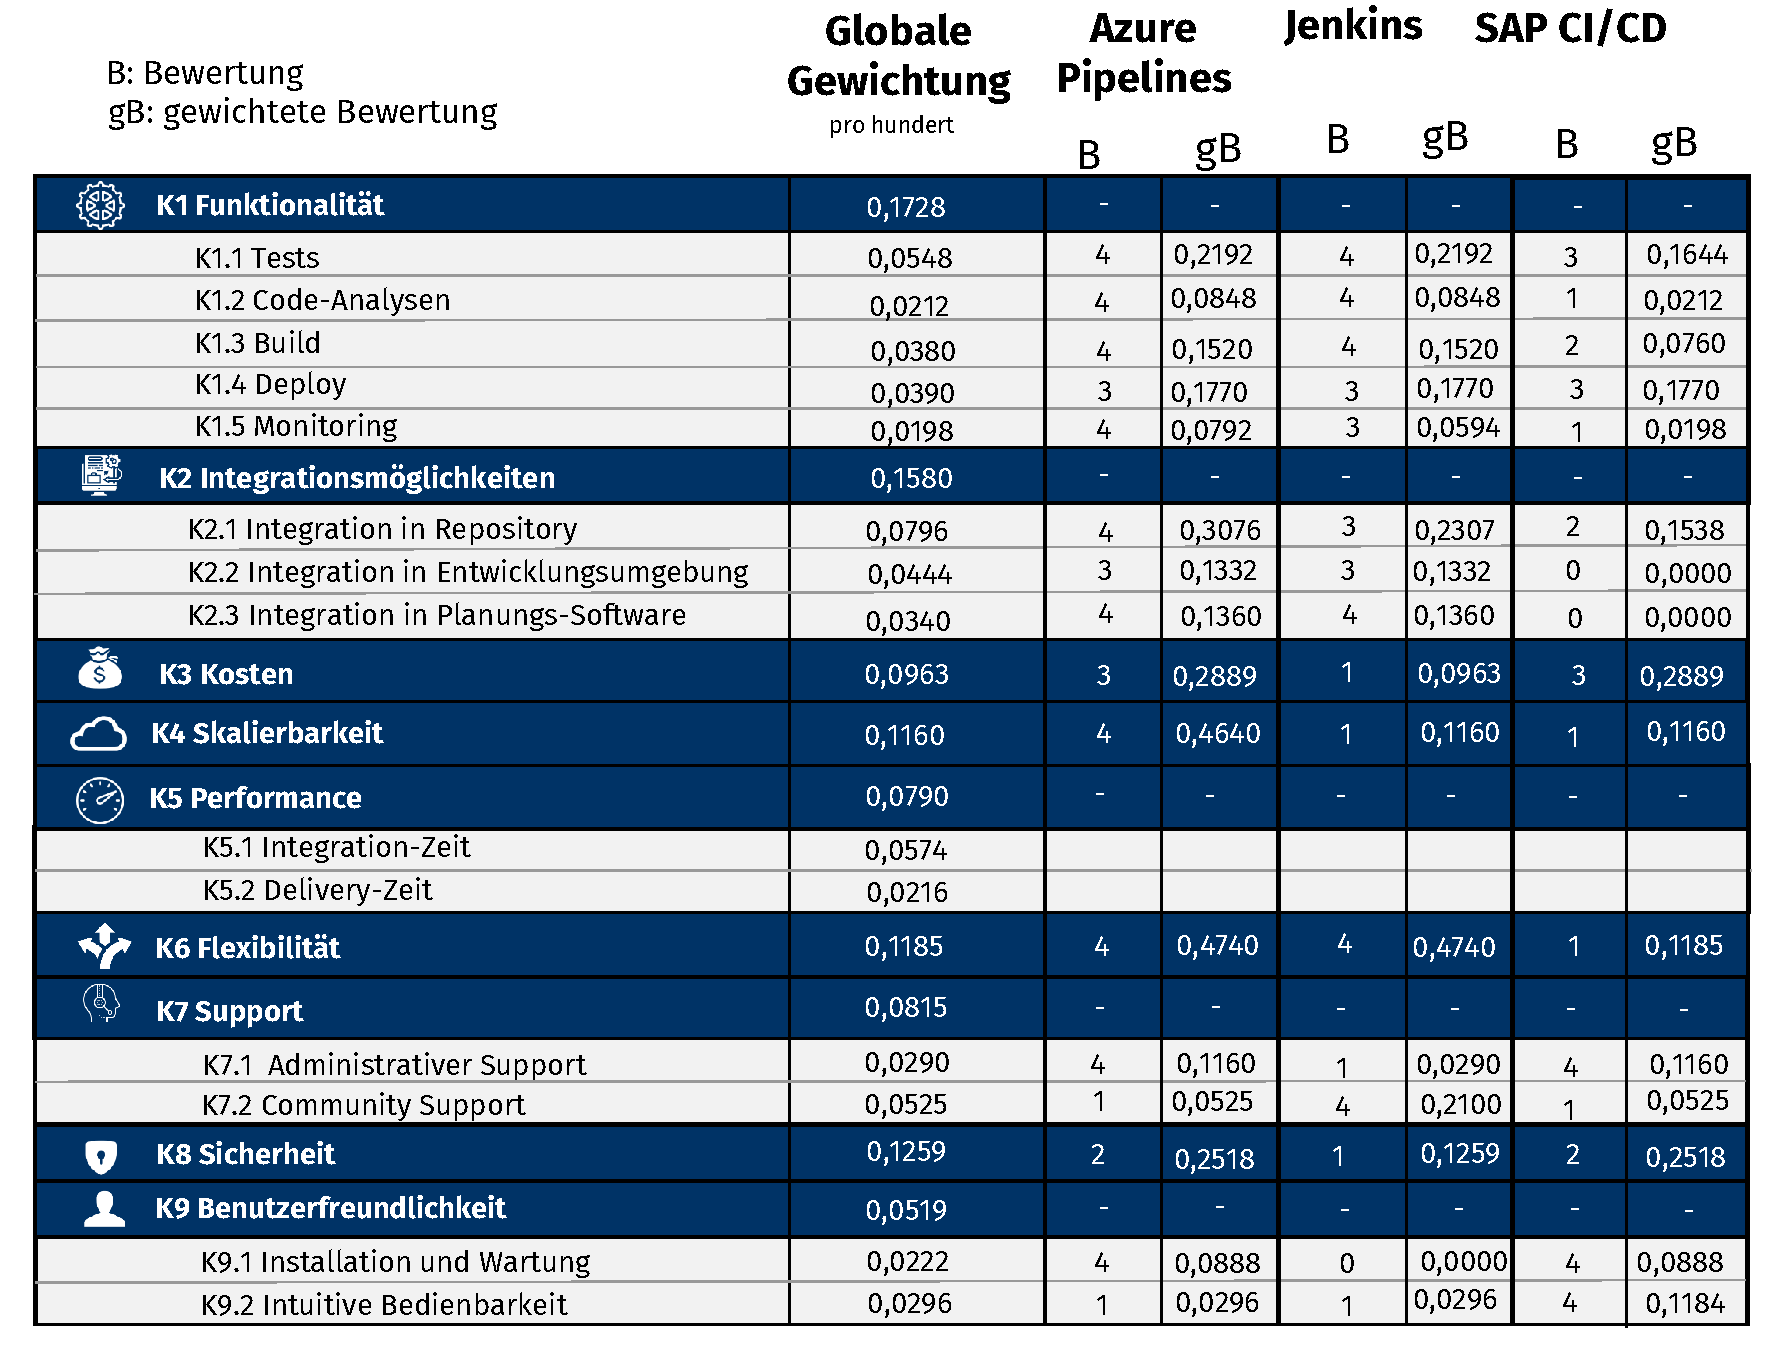
\includegraphics{Ergebnis}}
		\caption[Ergebnistabelle zum AHP]{Ergebnistabelle zum AHP. Eigene Darstellung.}
		\label{tab:Ergebnis}
	\end{table}
\end{center}
\vspace*{-15mm}
Unter Berücksichtigung der zu untersuchenden Fragestellung ergibt sich eine Gesamtbewertung von 4,0117 für Azure Pipelines, 2,2947 für Jenkins und 1,7349 für SAP CI/CD (s. Tab. \ref{tab:Ergebnis}). Somit kann Azure Pipelines auf Grundlage des in der Arbeit entworfenen Entscheidungs-Framework als das optimale CI/CD-Tool betrachtet werden.  

